\title{Machine Learning Practical - Assignment 4}
\author{s1247438}
\documentclass[12pt]{article}
\usepackage{caption}
\usepackage{subcaption}
\usepackage[pdftex]{graphicx} 
\usepackage[margin=1in]{geometry}    
\usepackage{float}

\begin{document}

\maketitle


\subsection*{Introduction}

This coursework continues to explore more advanced topics in Neural Networks following the work from the last assignment \cite{me}. The experiments are focused on the CIFAR-10 and CIFAR-100 datasets with a 40,000 training , 10,000 validation and 10,000 test split. These contain sets of 32x32 labeled images falling into 10 and 100 categories respectively. The investigated methods will try to improve upon the baseline model found in the previous coursework, taking advantage of what has been learned during the model development. The baseline model is listed in Table \ref{tab:baseline}, the main takeaways for further experiments are the number of layers, number of hidden units and data augmentation (horizontal reflection, random brightness, random contrast). 


\begin{table}[H]
\centering
\begin{tabular}[h]{| c | c |}
\hline
model & 3 Relu  \\
\hline
error & cross-entropy softmax   \\
\hline
hidden units per layer & 200   \\
\hline
learning rule & AdaGrad   \\
\hline 
data augmentation & horizontal reflection  \\
\hline
batch size & 50   \\
\hline
result accuracy C-10& 55\%   \\
\hline
\end{tabular} 
\caption{Baseline Model parameters}
\label{tab:baseline}
\end{table}

This coursework focuses on exploring topics regarding Convolutional Neural Networks(CNN) expecting a dramatic increase in performance that CNNs are reported to bring on image classification tasks\cite{inspiration}\cite{bestprac}\cite{frac}. More specifically the coursework will explore the following topics

\begin{itemize}
\item What is a well performing network architecture in terms of the number of convolution, pooling and fully connected layers? This  topic will use the previously learned baseline model as a starting point expecting to reach a conclusion in terms of number of layers similar to what papers exploring CIFAR suggest \cite{inspiration}. A good model architecture is needed for further topics to be explored.
\item Can further data augmentation prevent over-fitting? Despite the data aumentations explored the previous model was still prone to overfitting. One approach that has not been explored in the previous model but reported as benefical is random cropping\cite{kernel}\cite{crop}
\item What is an appropriate convolution filter size and stride? This question will expect to arrive to the same conclusions as many papers suggesting only few reasonable values for these \cite{inspiration}\cite{bestprac}\cite{frac}.
\item What is an appropriate pooling type, kernel size and stride? As with the question above the expectation is to default to standard values. For this reason the question will further explore the possible benefits of fractional pooling as suggested by a recent paper\cite{frac} over max pooling.
\item How does the performance of an all convolutional network\cite{allconv} compare? The all convolutional network replaces pooling layers by convolution layers with stride 2 and reports similar results as network with pooling layers. 
\end{itemize}

\subsection*{Implementation}

The code for exploring Convolutional Neural Networks is an adaptation from the official tensorflow tutorial\cite{tf}. The tutorial code was chosen as a basis over the one developed for the previous model and given data provider for performance and structure reasons. The tutorial code takes advantages of multi-threaded way of creating queues using \textit{tf.train.batch()} and more efficient methods for data augmentation from \textit{tf.image} library. The code also uses \textit{tf.train.MonitoredTrainingSession} and hooks to output data during training which seems as a better practice, as well as better integration with tensorboard and storing checkpoints. Taking advantage of \textit{tf.app.flags} the model can be instructed from the command line to what to parameters to test, improving scalability.  This code was then adapted to work on a basis of epochs rather than step and tracking accuracy and loss on a per epoch basis. The LoggerHook attached to the MonitoredTrainingSession keeps track of undertaken steps and therefor epochs. On each epoch it stores the training accuracy and loss per epoch, as well as runs a validation script that loads the last stored model and stores the validation accuracy and loss. These can be later easily compared in tensorboard. This code was then deployed on Amazon AWS p2.xlarge GPU instance taking 60-100 seconds per epoch.



\subsection*{Methods}

\subsubsection*{Network Architecture}

Various network architectures were explored mainly the number of convolution and pooling layers. The model found in previous coursework depicted on Table \ref{tab:baseline} was used as both a baseline and the fully connected layers. Three fully connected layers of 200 hidden units each were used at the start. Explored models were trained on an augmented dataset (flip,contrast,brightness).The experiments consisted of iteratively adding convolution and pooling layers before the fully connected ones taking advantage of the tensorflow functions \textit{tf.nn.conv2d(input, filter, strides, padding, usecudnnongpu=None, dataformat=None, name=None)} and \textit{tf.nn.maxpool(value, ksize, strides, padding, dataformat='NHWC', name=None)}. However these functions require parameters for filter, stride and kernel size values. The effect of these and an appropriate choice will be explored in the latter sections. The initial values for these were taken from a paper which had a well performing model for CIFAR \cite{inspiration} displayed on Table \ref{tab:convpoolpar}. The maximum number of convolution and pooling layers were three as after 3 pooling layers the resulting data size was too small for the chosen kernel size. 

\begin{table}[H]
\centering
\begin{tabular}[h]{| c | c |}
\hline
Filter size & 5  \\
\hline
Filter stride & 1   \\
\hline
Number of filters & 64   \\
\hline
Kernel size & 3   \\
\hline 
Kernel stride & 2   \\
\hline 
Batch size & 128   \\
\hline 
\end{tabular} 
\caption{Initial parameters for Convolution and Pooling layers}
\label{tab:convpoolpar}
\end{table}

The results of different architectures are displayed on Figure \ref{fig:arch}. All models were run only for 30 epochs due to computational complexity, relaying that the number of epochs will be enough to compare architectures and see trends occurring. These show a significant improvement on validation set accuracy over the non-covolutional baseline model which achieved 58\% and the 3 convolution and pooling layers coupled with two fully connected layers of 200 hidden units achieved 81\% accuracy in just 30 epochs. This architecture will be used across the next sections.

\begin{figure*}[ht!]
    \centering
    \begin{subfigure}[t]{0.475\textwidth}
        \centering
        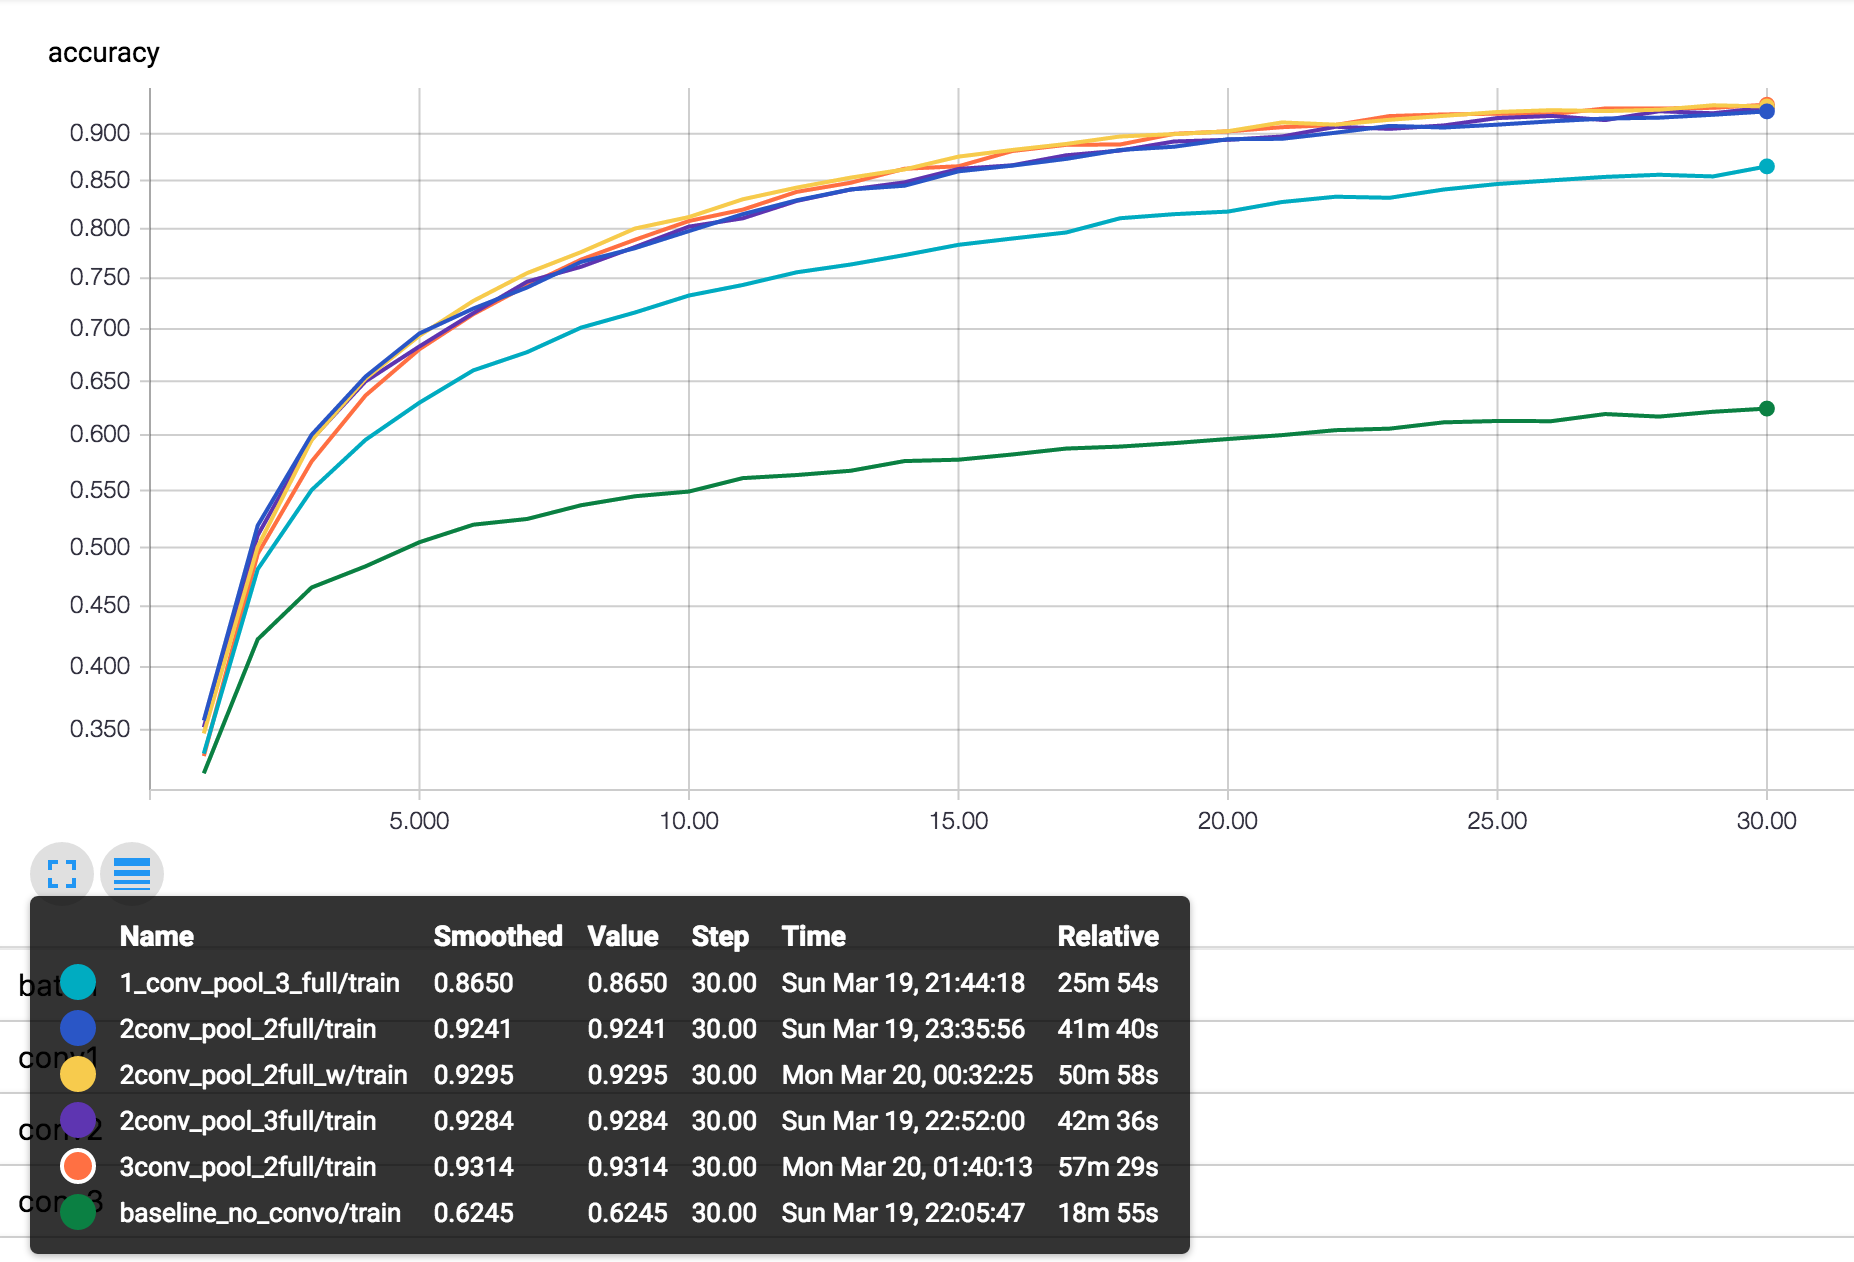
\includegraphics[width=1.0\linewidth]{netowrkacct.png}
    \end{subfigure}%
    ~ 
    \begin{subfigure}[t]{0.475\textwidth}
        \centering
        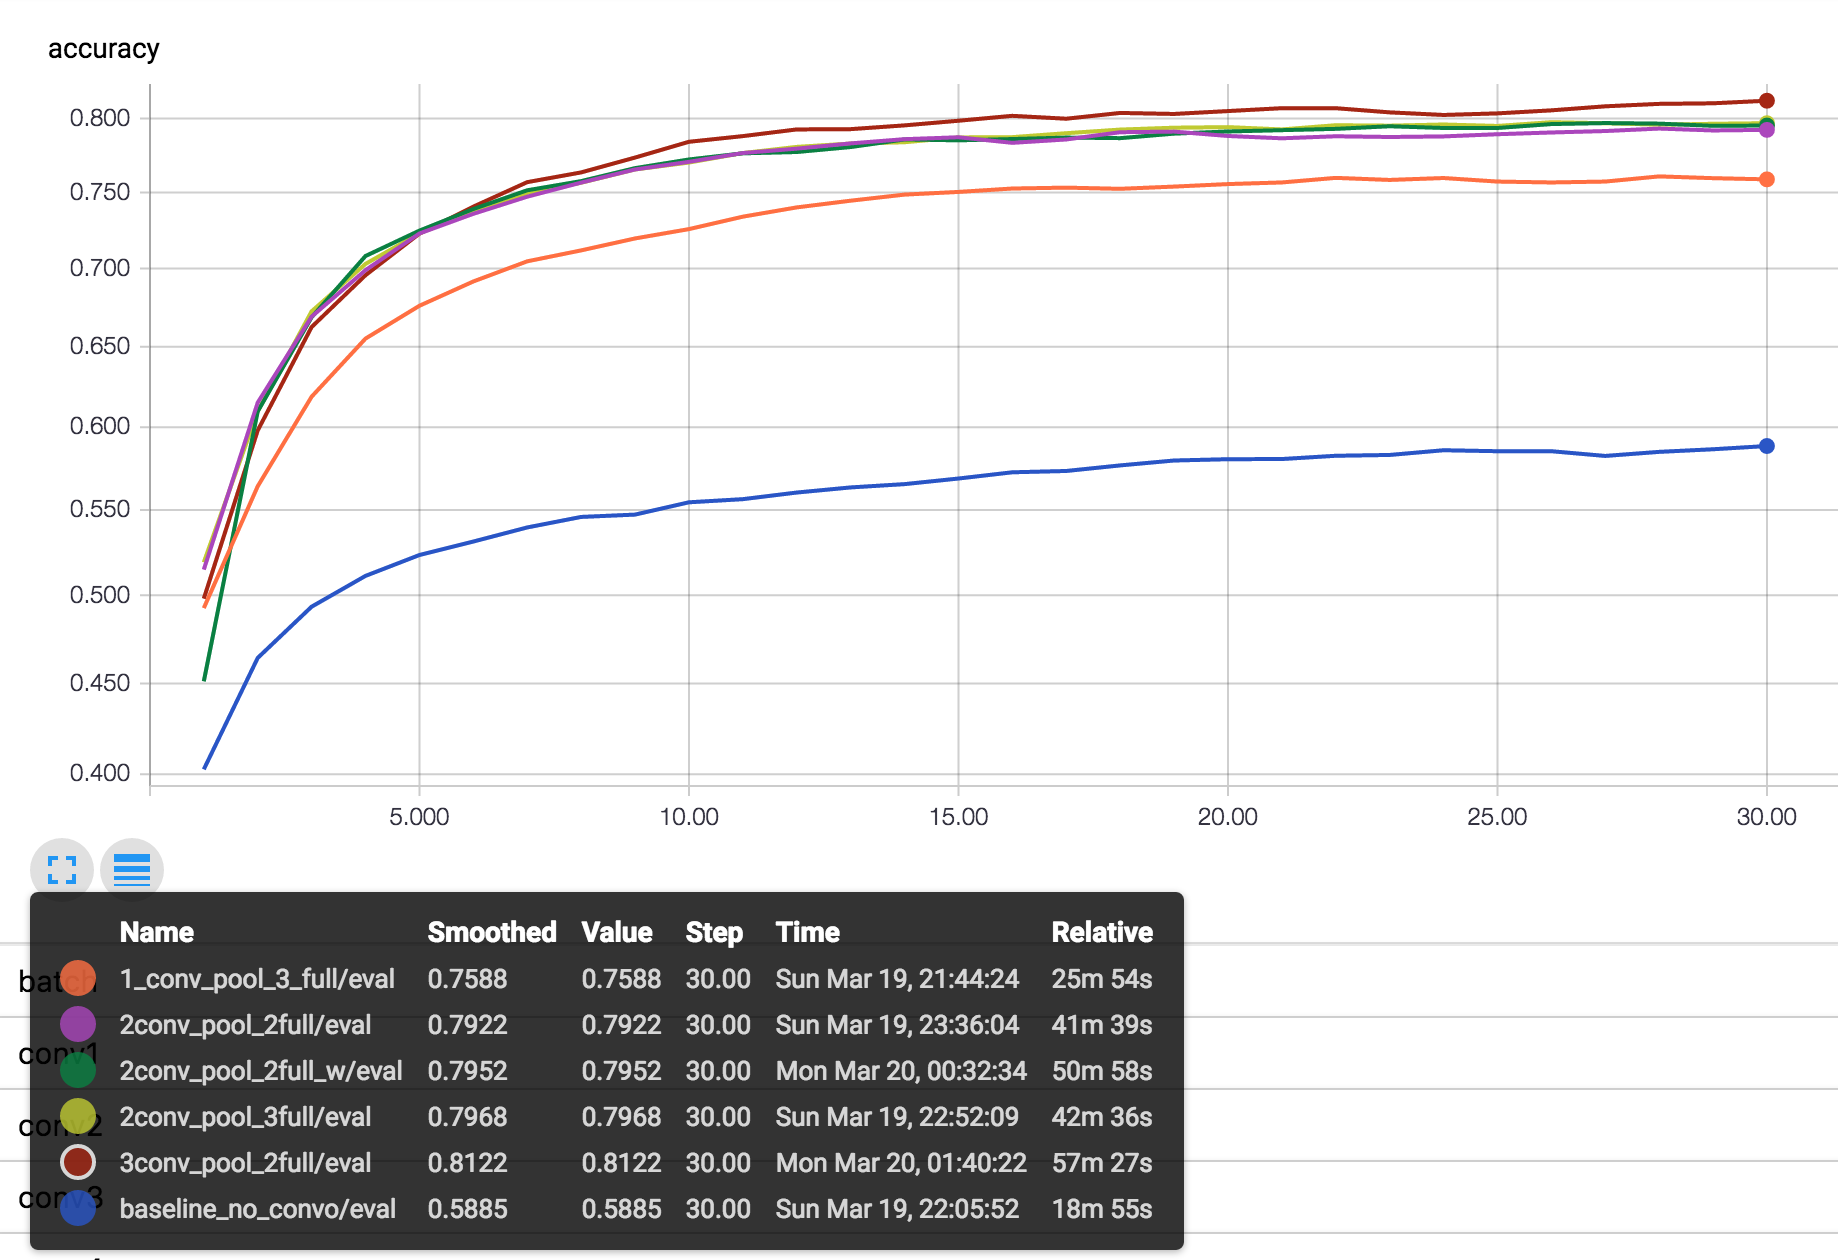
\includegraphics[width=1.0\linewidth]{networkacc.png}
    \end{subfigure}
    \caption{Comparison of different architecture model accuracies for 30 epochs, training set on the left and validation on the right. Highlighting the best performing one}
    \label{fig:arch}
\end{figure*}

\subsubsection*{Data Augmentation}

Previous coursework\cite{me} explored various data augmentation methods and found flipping, brightness and contrast to be effective in decreasing the level of over-fitting and improving accuracy. Exploring the graphs on Figure \ref{fig:noaug} one can see the model is still over-fitting to the training data. One popular data augmentation method mentioned in a number of papers \cite{kernel}\cite{crop} is random cropping. This section explored performing a random 24x24 crop of the original 32x32 images using \textit{tf.random\_ crop()}, achieving a significant increase of the training data.

\begin{figure*}[ht!]
    \centering
    \begin{subfigure}[t]{0.475\textwidth}
        \centering
        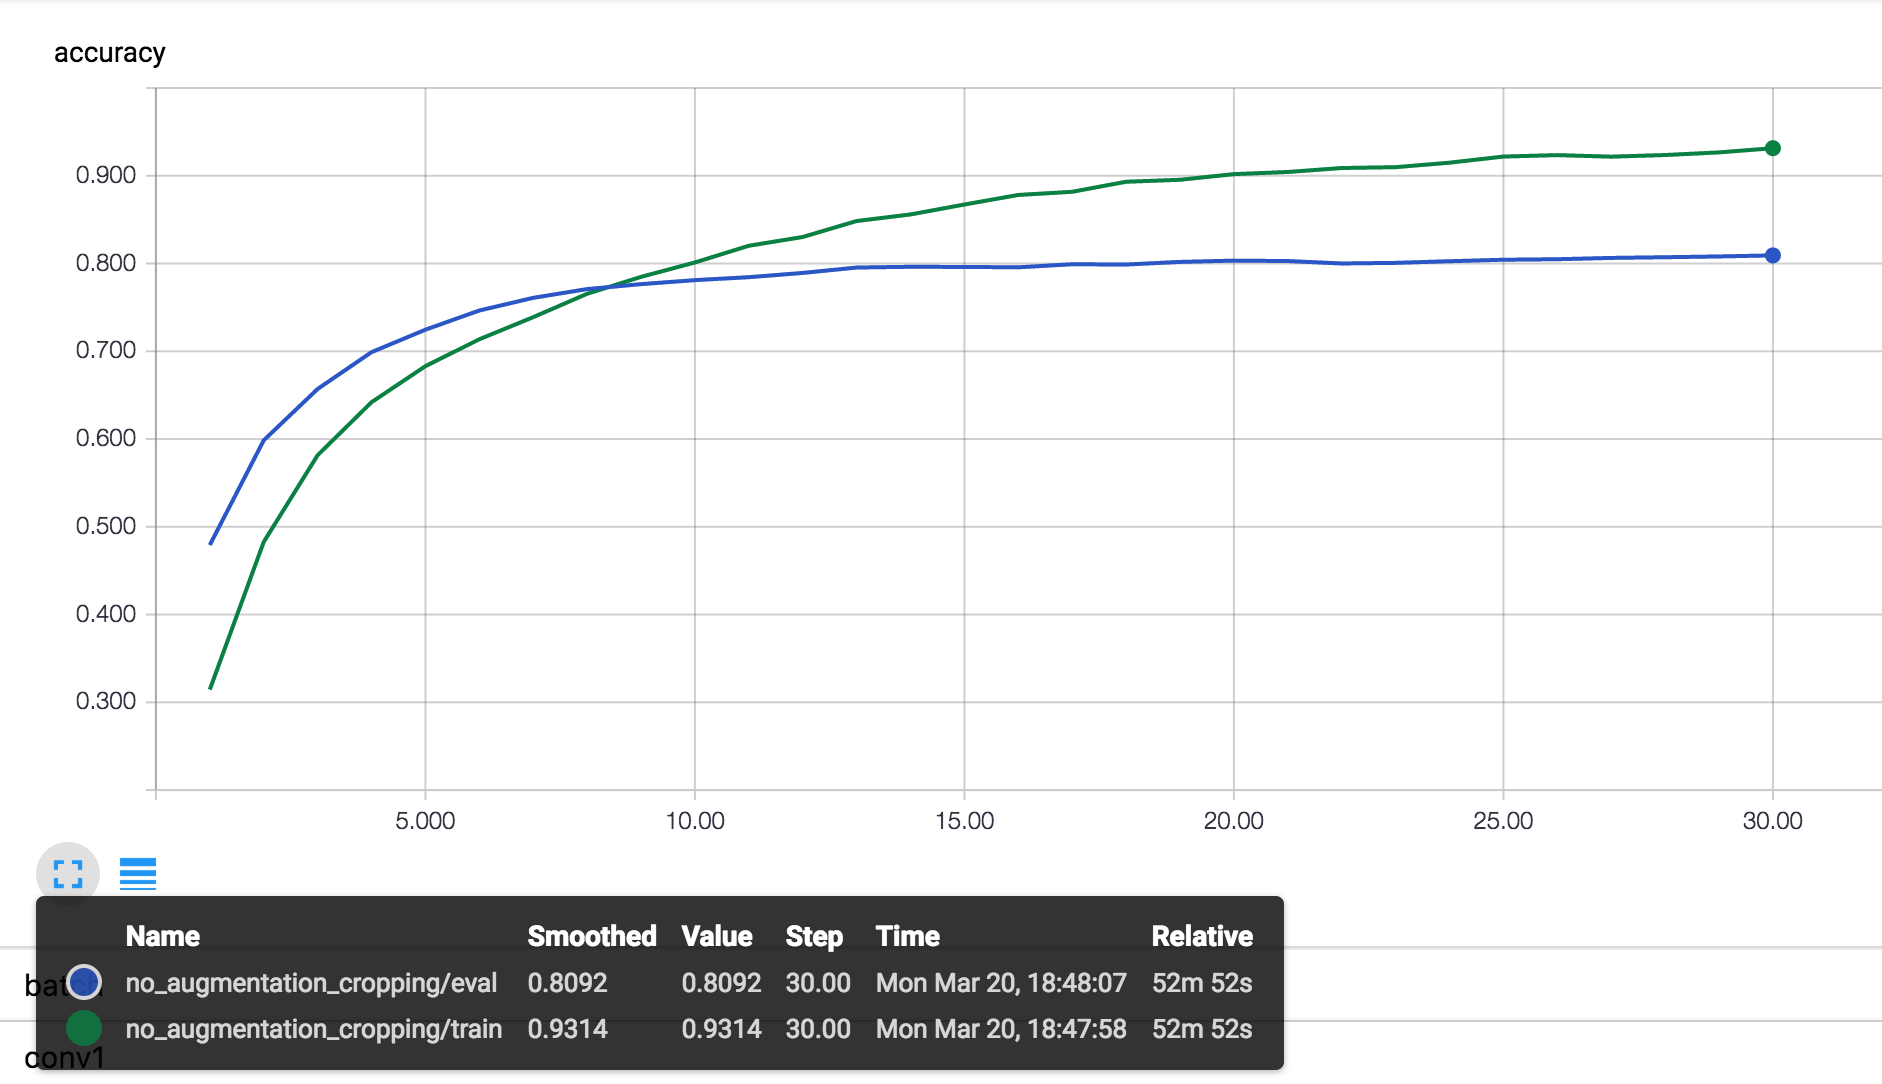
\includegraphics[width=1.0\linewidth]{noauga.png}
    \end{subfigure}%
    ~ 
    \begin{subfigure}[t]{0.475\textwidth}
        \centering
        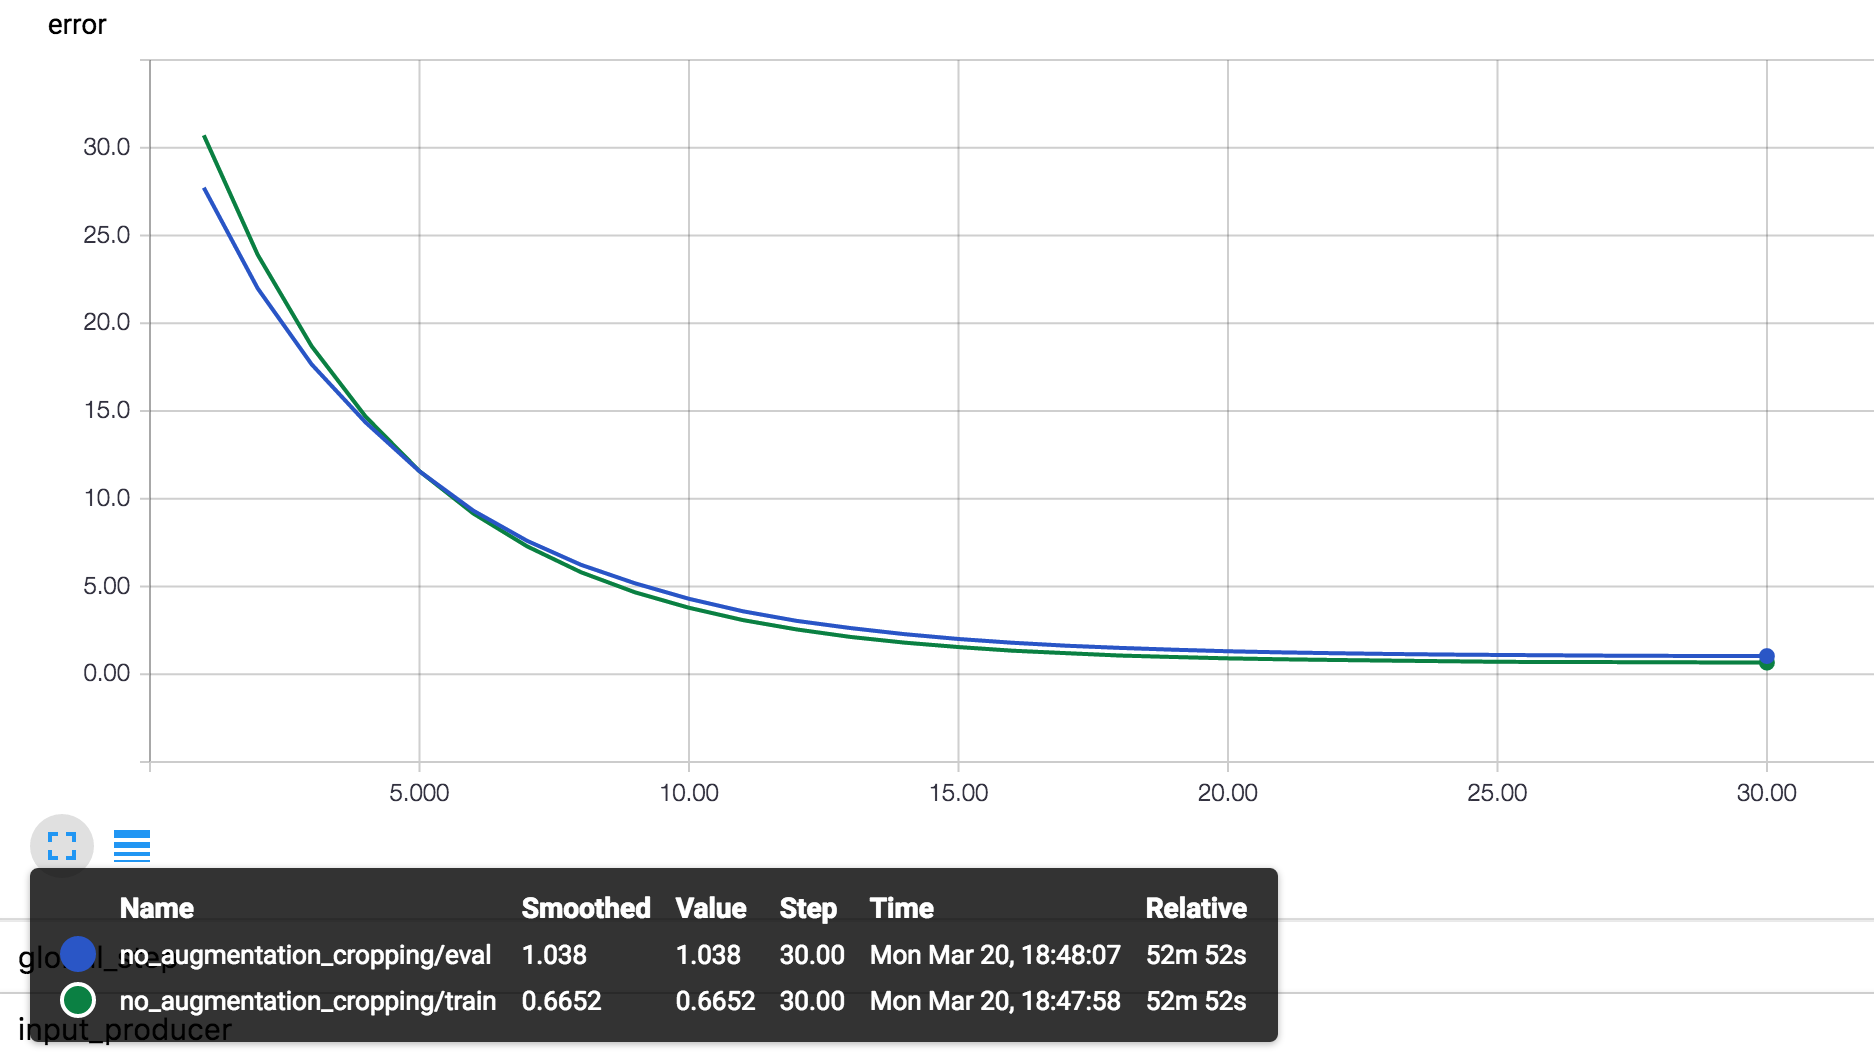
\includegraphics[width=1.0\linewidth]{noaugt.png}
    \end{subfigure}
    \caption{Model performance without random cropping data augmentation showing over-fitting. }
    \label{fig:noaug}
\end{figure*}

Figure \ref{fig:aug} shows the effects of random cropping data augmentation. The model learns a little slower but even in the small number of epoch matches and starts overtaking the classification performance of the one without random cropping. The model results in a higher validation than training accuracy clearly benefiting with the essentially larger dataset.

\begin{figure*}[ht!]
    \centering
    \begin{subfigure}[t]{0.475\textwidth}
        \centering
        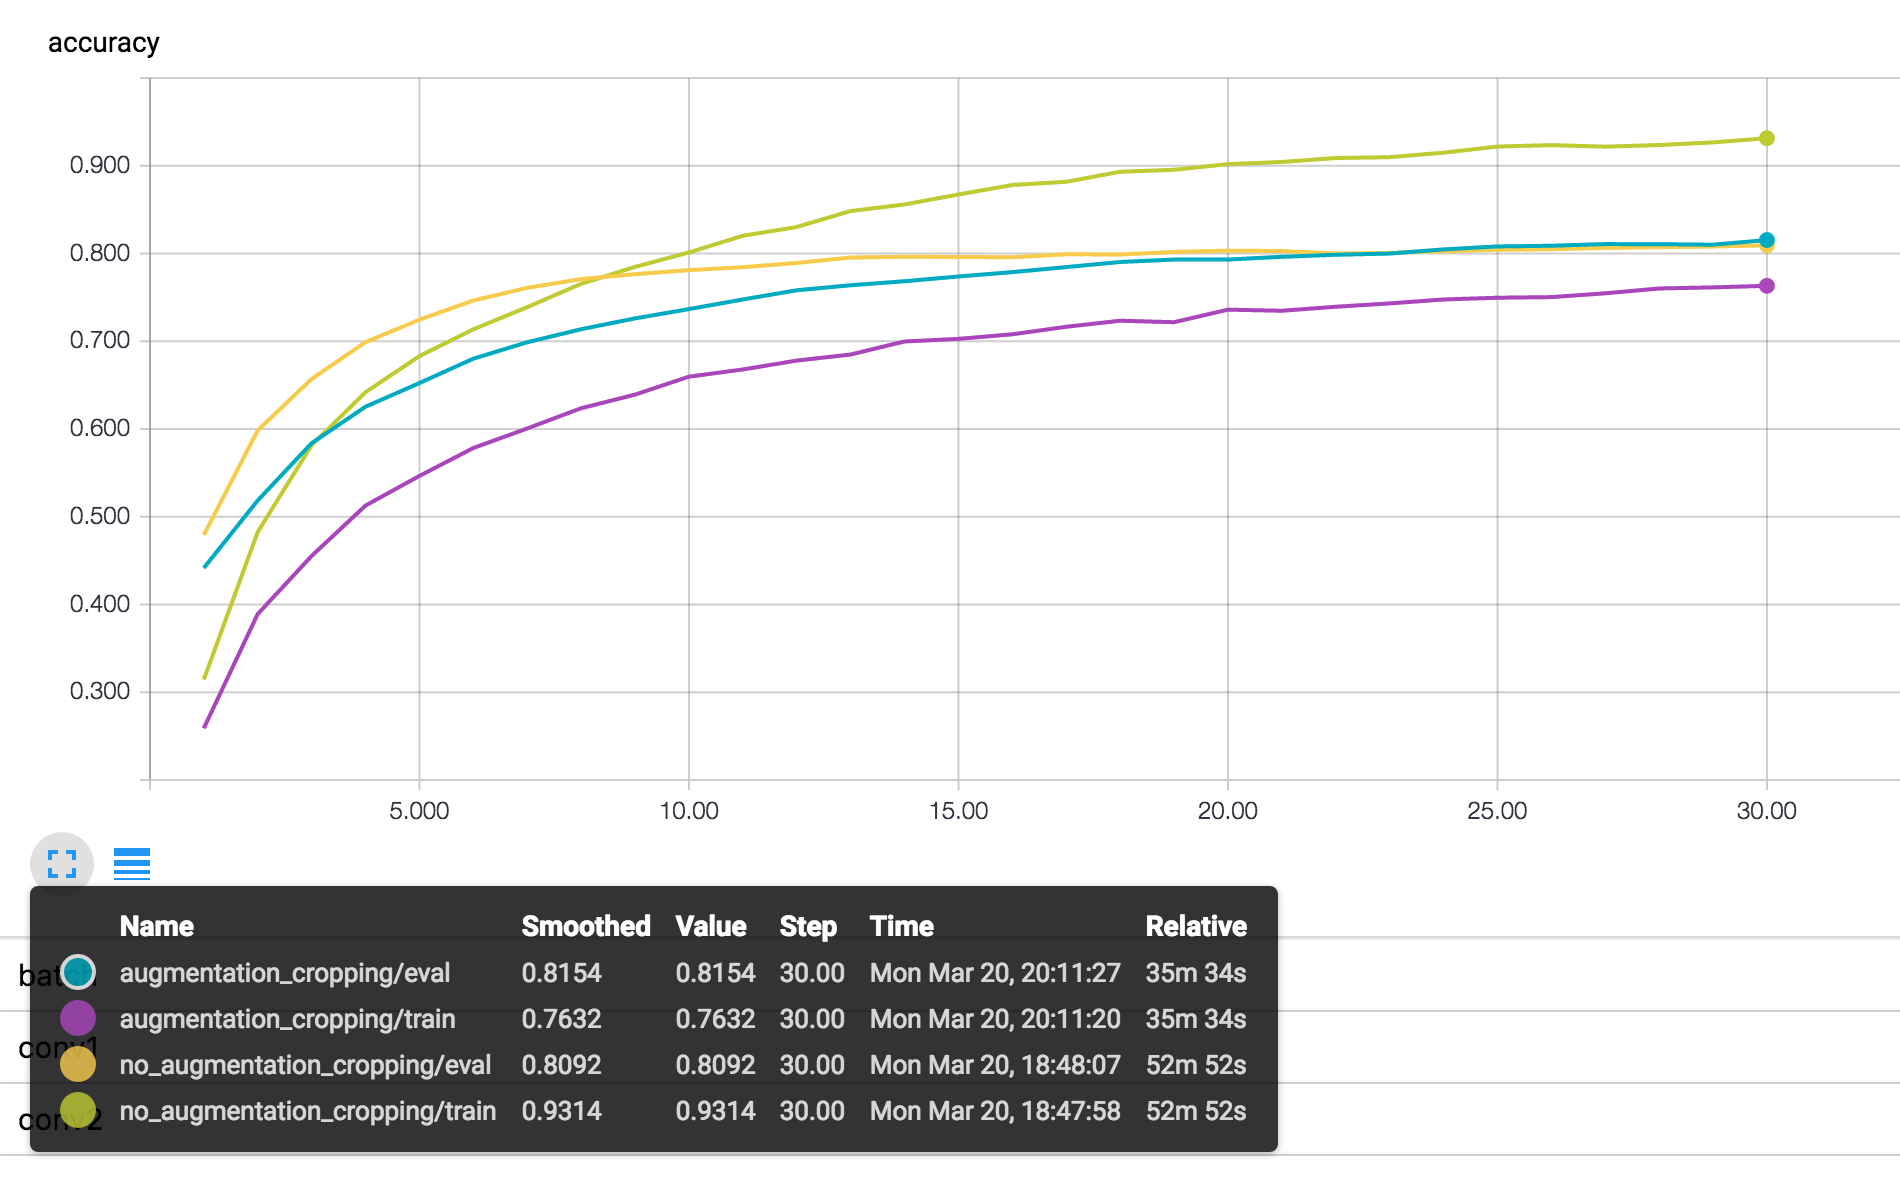
\includegraphics[width=1.0\linewidth]{auga.png}
    \end{subfigure}%
    ~ 
    \begin{subfigure}[t]{0.475\textwidth}
        \centering
        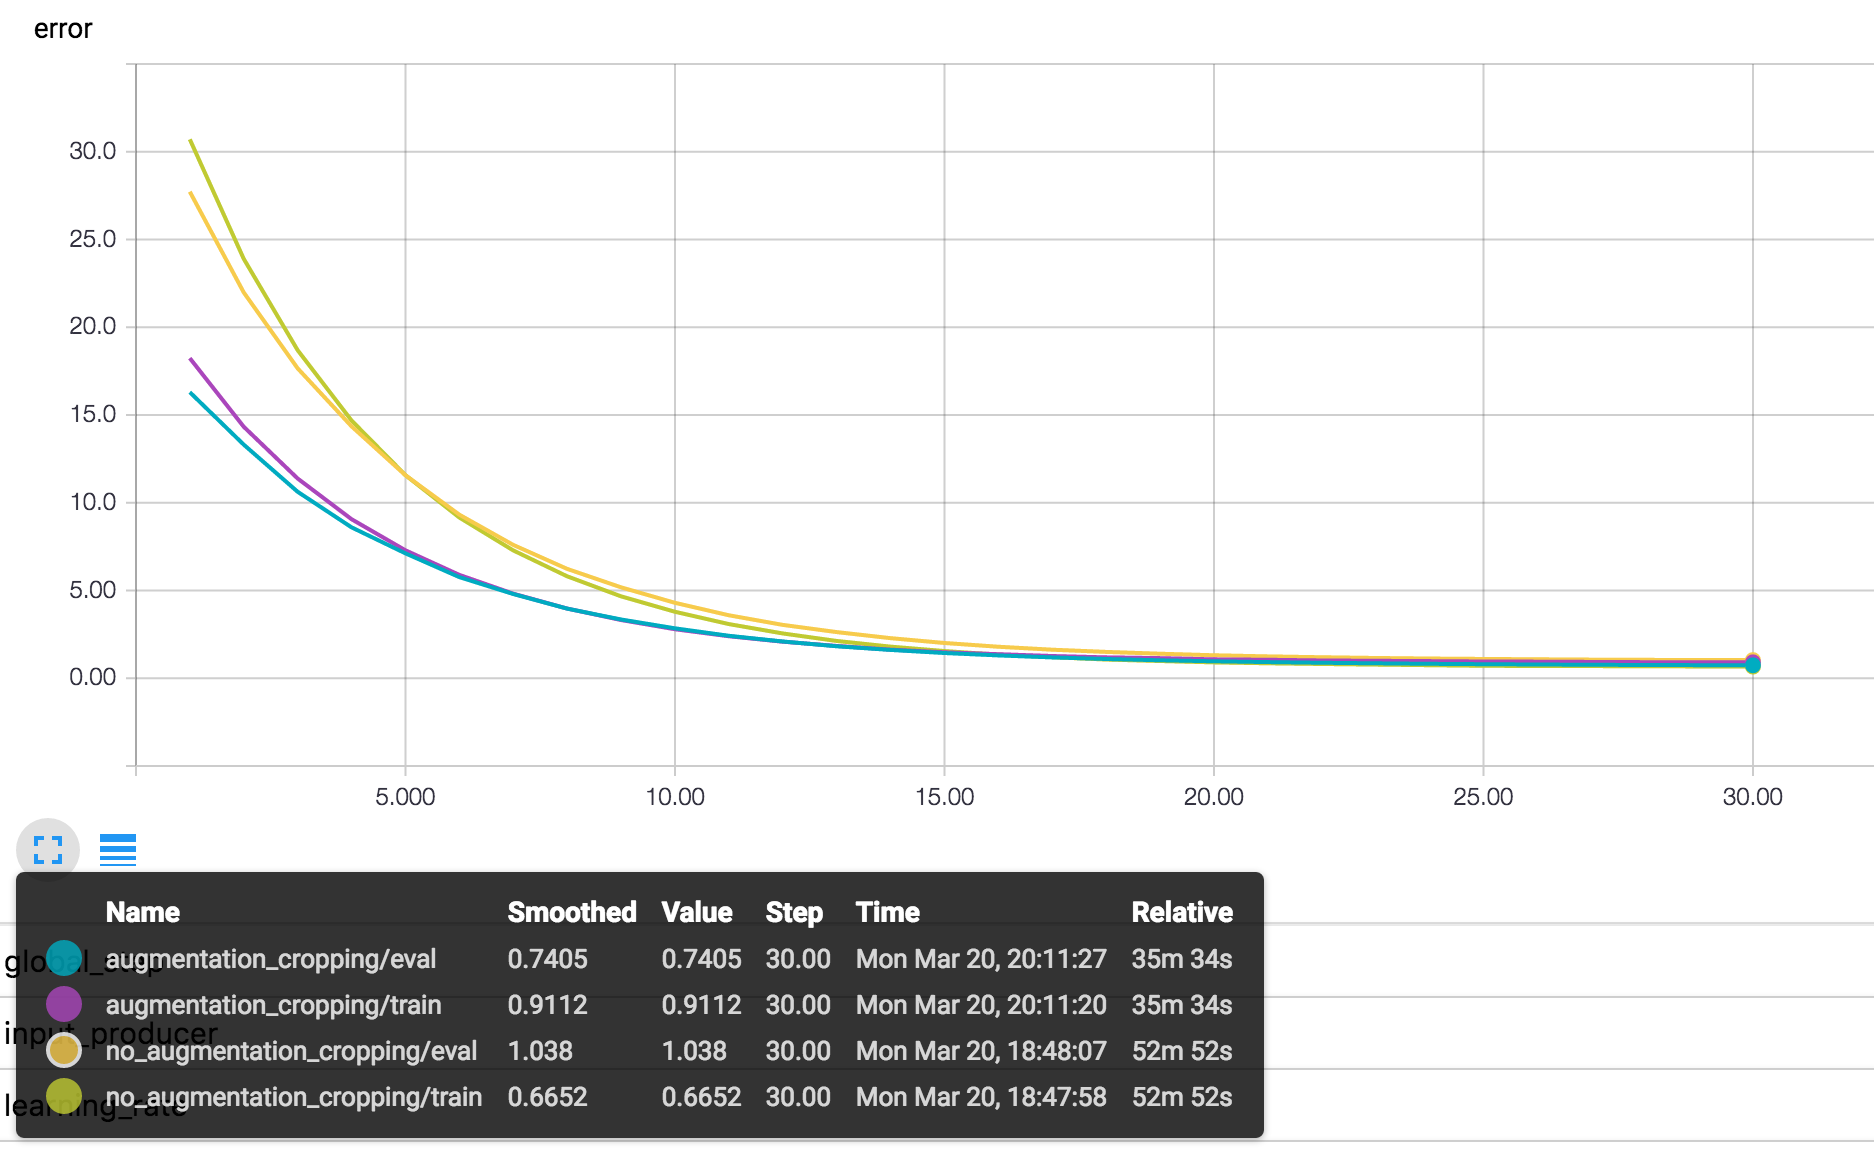
\includegraphics[width=1.0\linewidth]{augt.png}
    \end{subfigure}
    \caption{Model performance with random cropping data augmentation. }
    \label{fig:aug}
\end{figure*}

\subsubsection*{Convolution filter size and stride length}

Papers\cite{kernel}\cite{inspiration}\cite{bestprac} mentioning models on CIFAR and others often suggest a 5x5 filter size. The Stanford class on Convolutional Neural networks\cite{stan} similarly suggests using a 3x3, 5x5 or 7x7 filters with a stride of 1. A larger filter sizes are described as uncommon, AlexNet\cite{alexnet} used a filter size of 11x11 on the first convolutional layer, but the size of their input for ImageNet was much larger 224x224. This section experiments with the smaller filter sizes and strides. The results are shown on Figure \ref{fig:filter} confirming the initial hypothesis and suggesting a 3x3 or 5x5 filter with stride 1 is a reasonable choice. 

\begin{figure*}[ht!]
    \centering
    \begin{subfigure}[t]{0.475\textwidth}
        \centering
        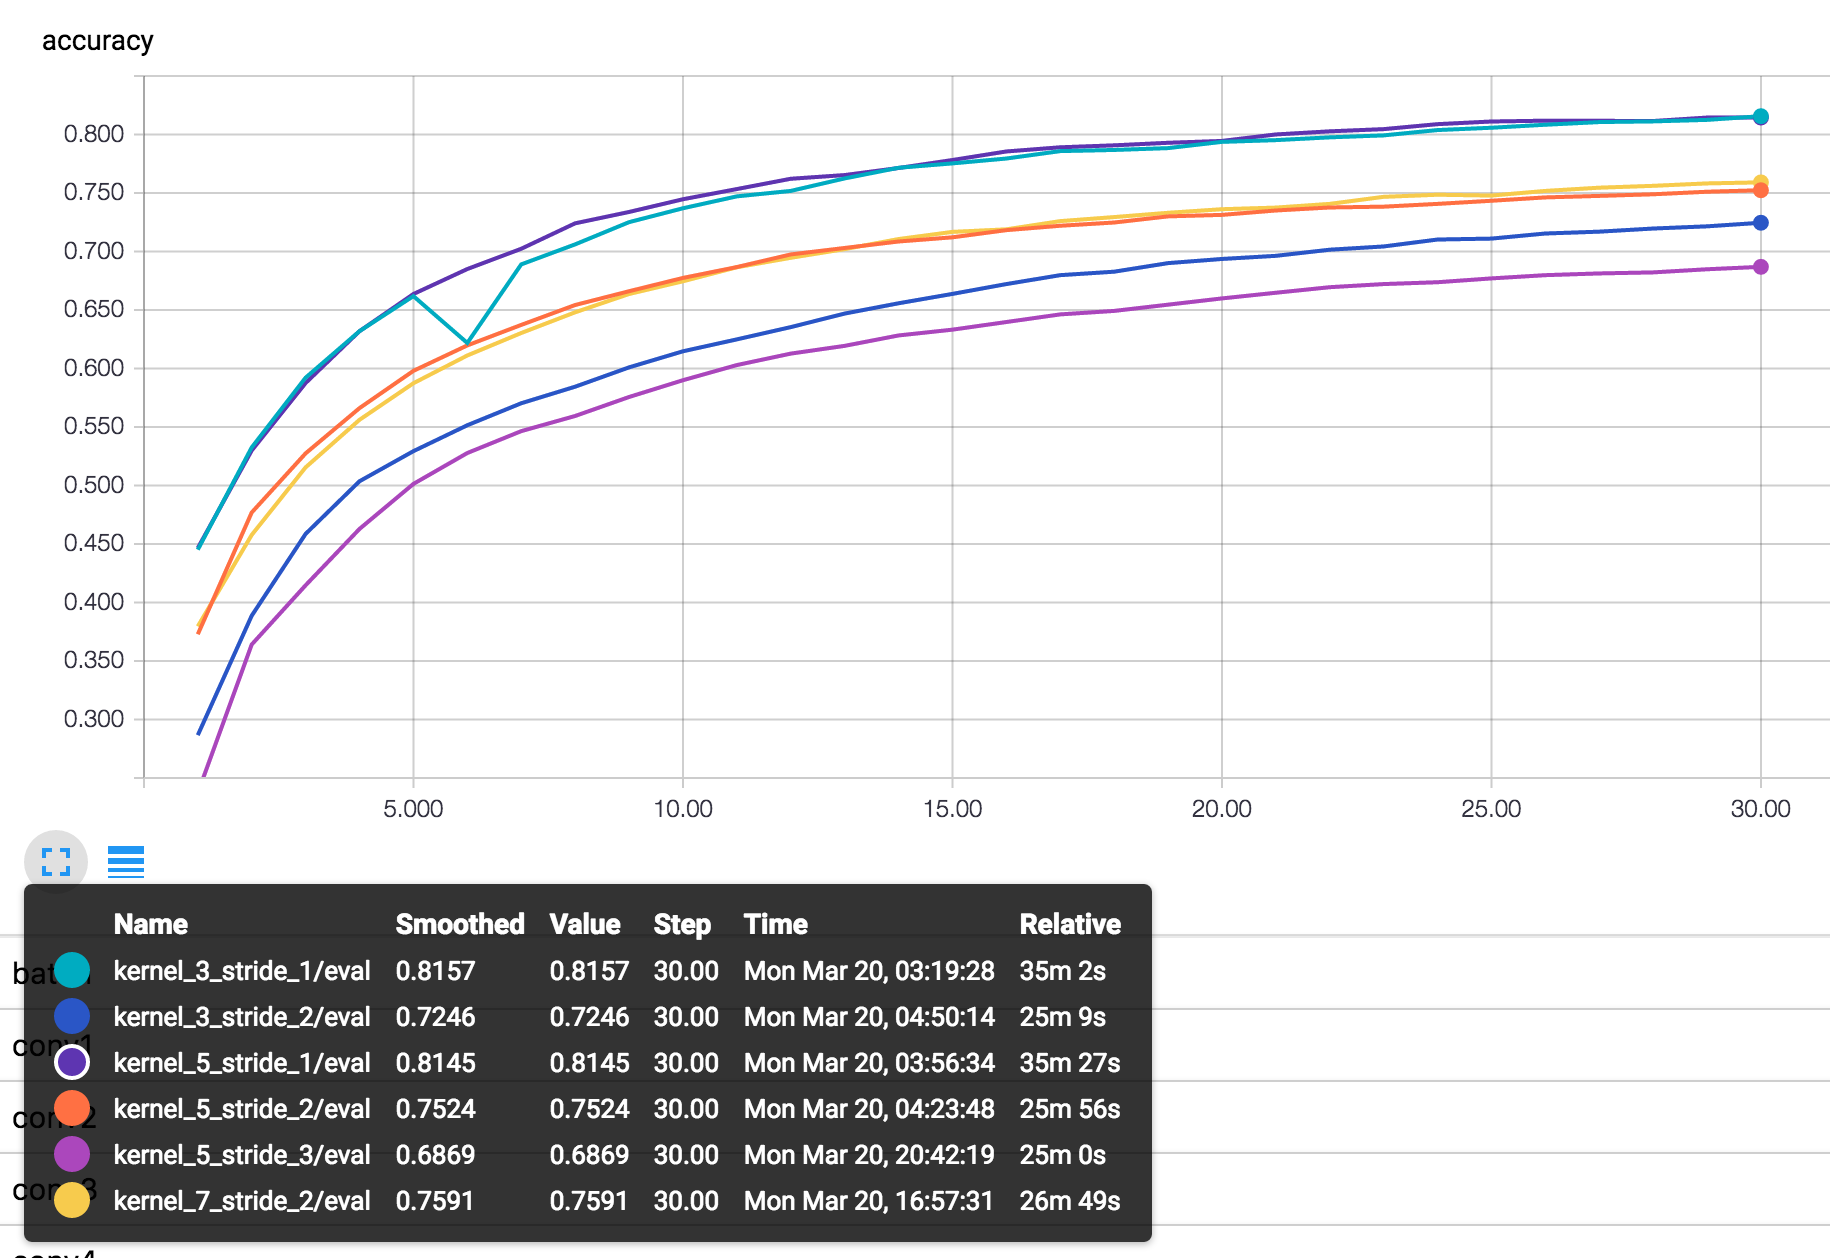
\includegraphics[width=1.0\linewidth]{filtera.png}
    \end{subfigure}%
    ~ 
    \begin{subfigure}[t]{0.475\textwidth}
        \centering
        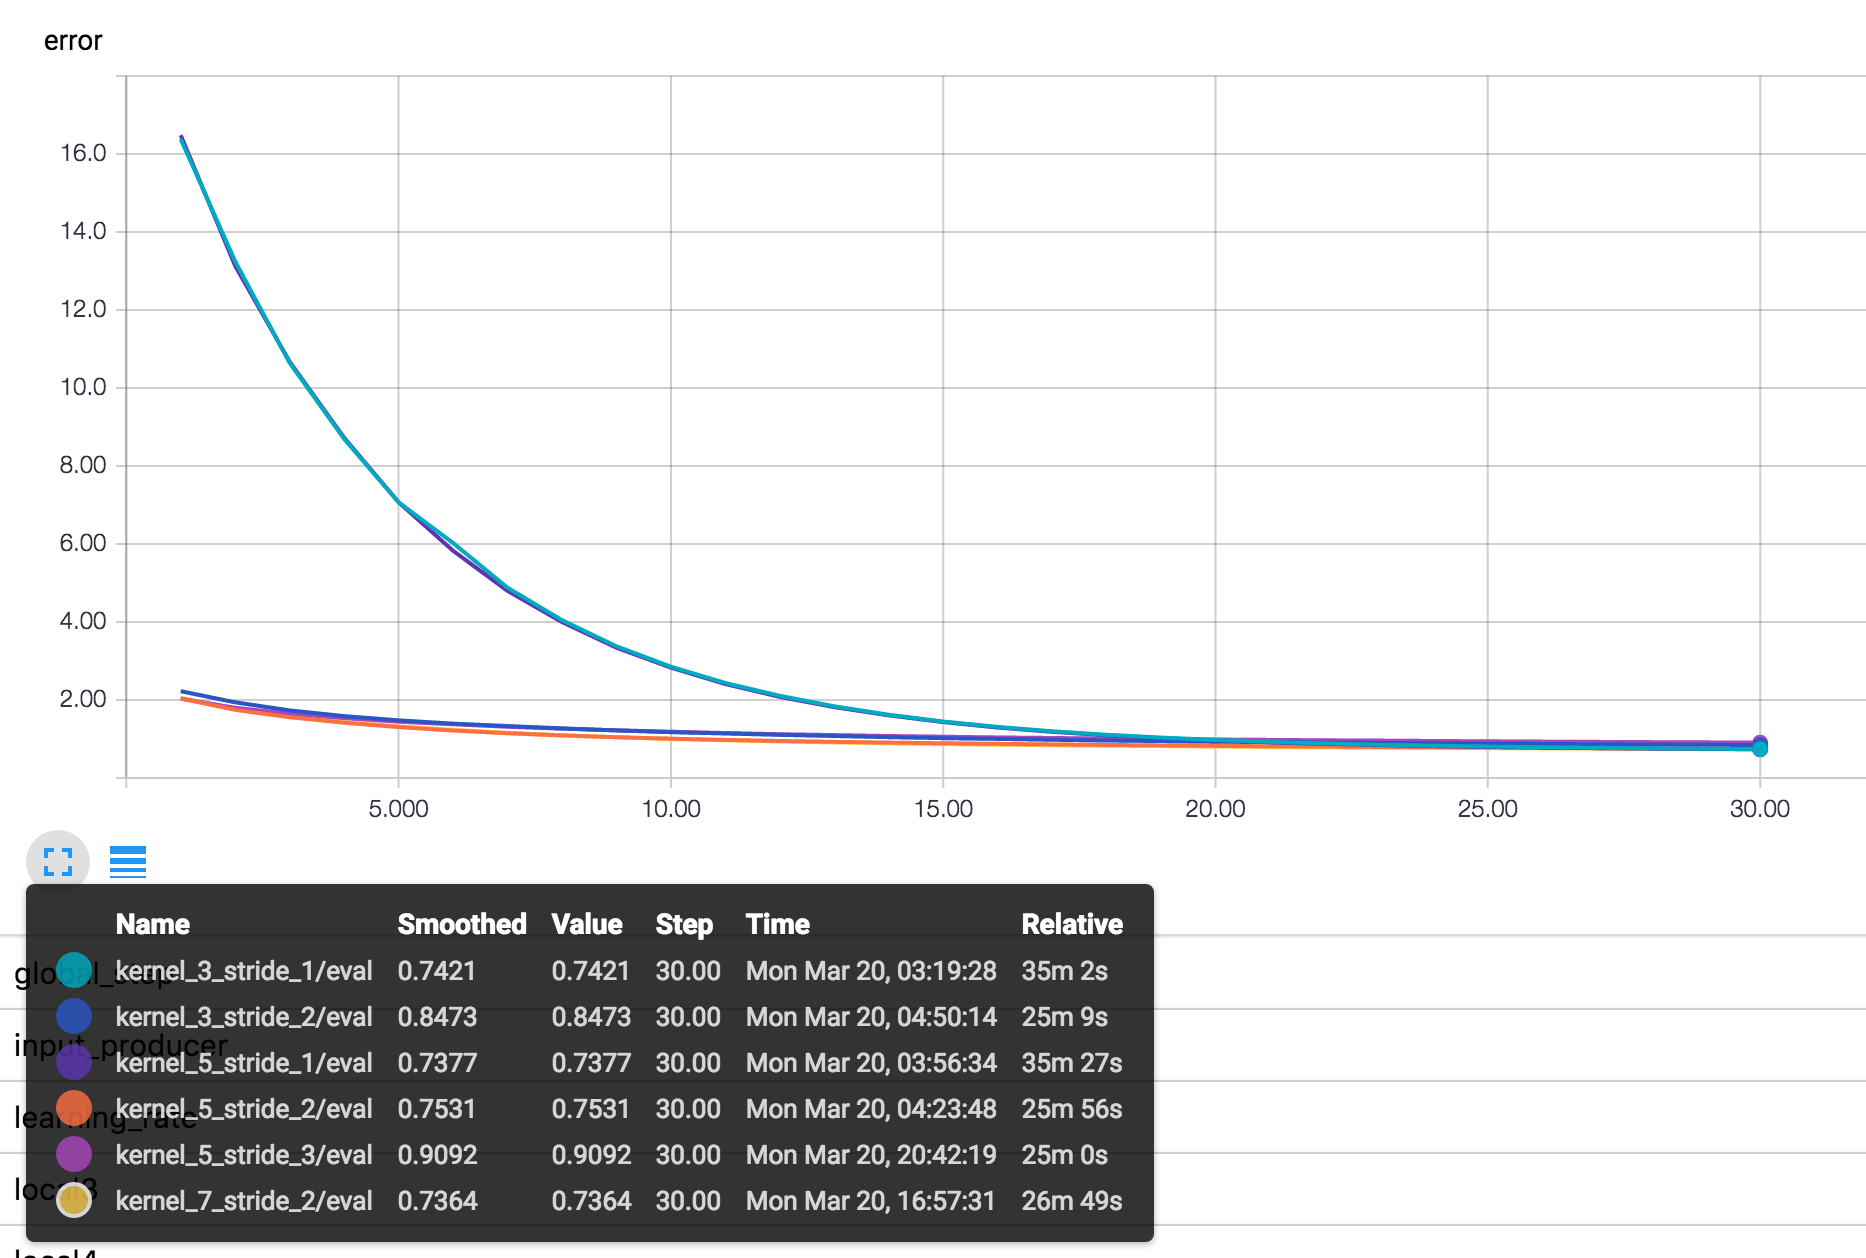
\includegraphics[width=1.0\linewidth]{filtere.png}
    \end{subfigure}
    \caption{Model performance on validation set with various filter sizes and stride lengths. }
    \label{fig:filter}
\end{figure*}


\subsubsection*{Pooling kernel size, stride length and fractional pooling}

Similarly as with the section above the common kernel sizes and stride lengths suggested\cite{kernel}\cite{inspiration}\cite{stan} and used are size 2x2 or 3x3 and stride 2 for max pooling. Max pooling was implemented using \textit{tf.nn.max\_ pool()} and the expected results are that overlapping pooling 3x3 with stride 2 will perform better than non-overlapping 2x2 kernel with stride 2\cite{frac}. The results are shown in Figure \ref{fig:pool}.

\begin{figure*}[ht!]
    \centering
    \begin{subfigure}[t]{0.475\textwidth}
        \centering
        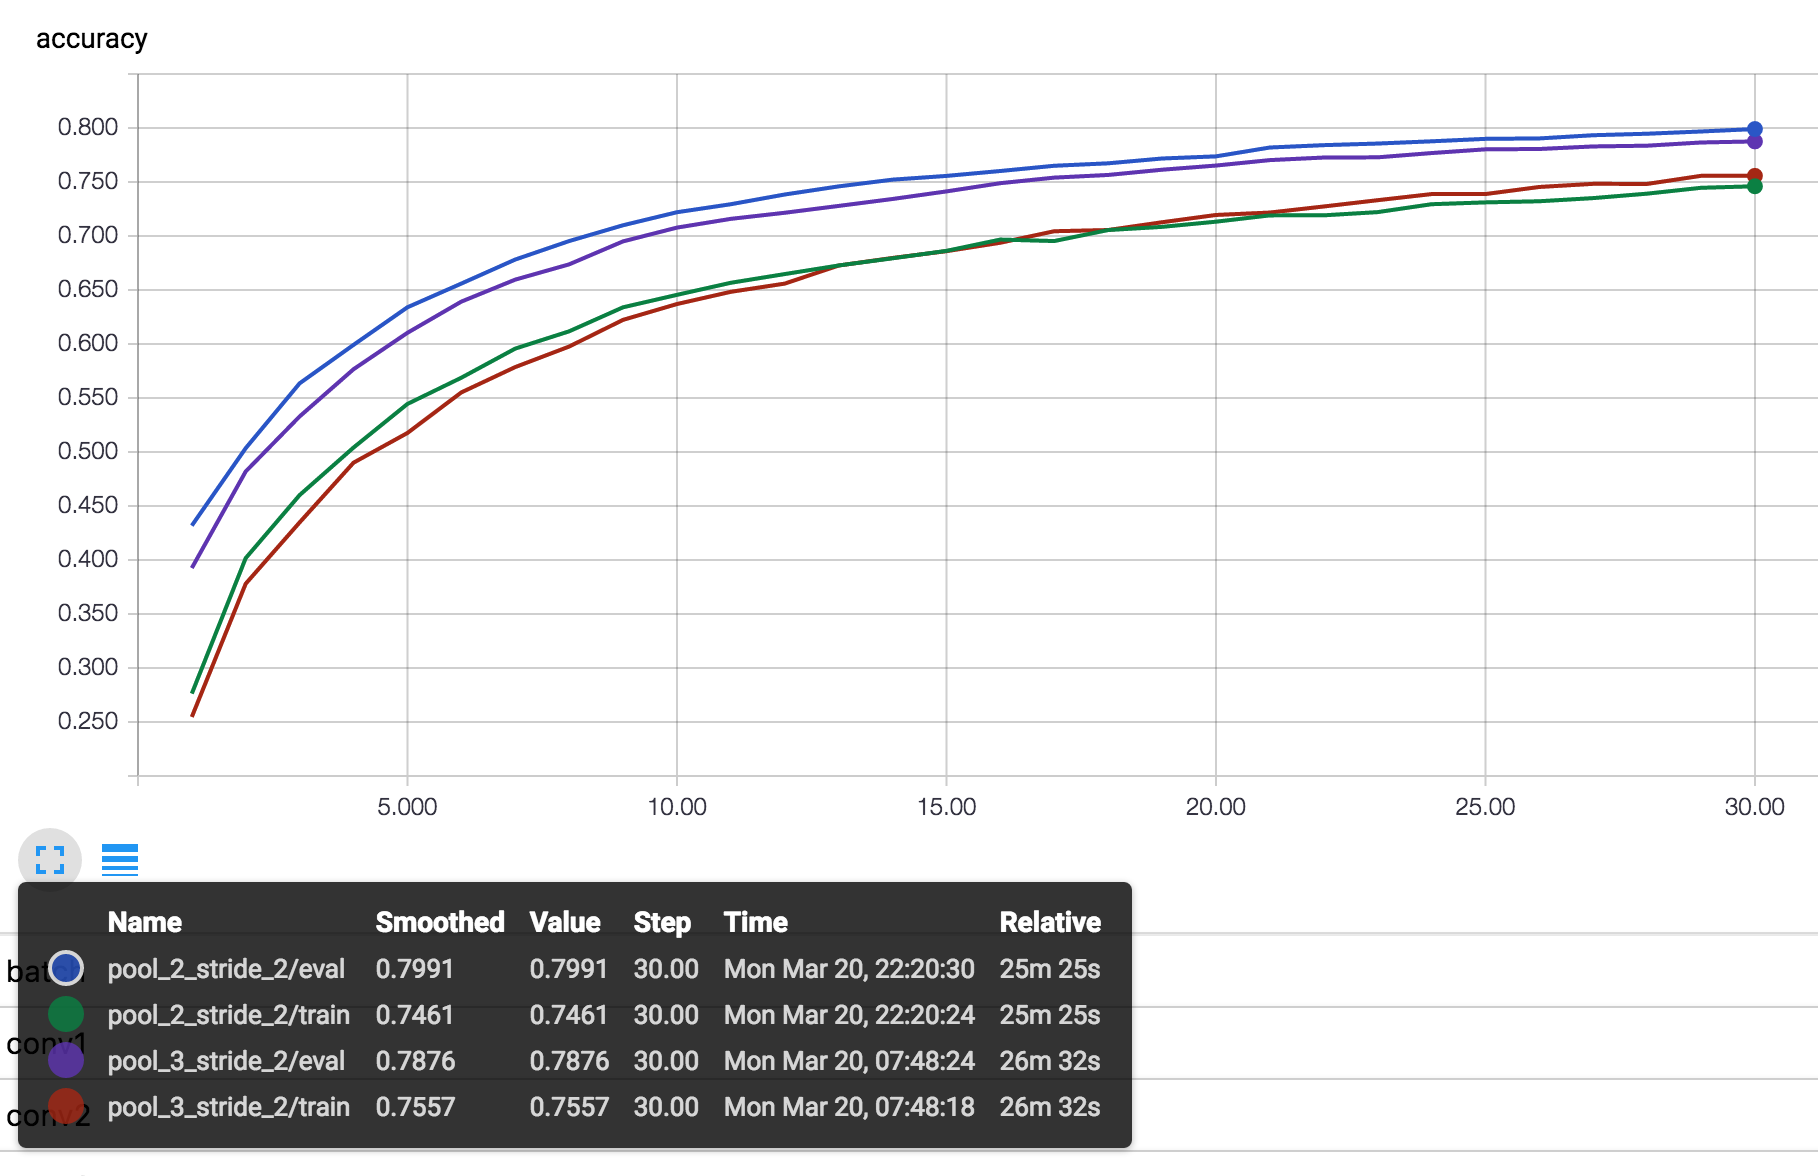
\includegraphics[width=1.0\linewidth]{poola.png}
    \end{subfigure}%
    ~ 
    \begin{subfigure}[t]{0.475\textwidth}
        \centering
        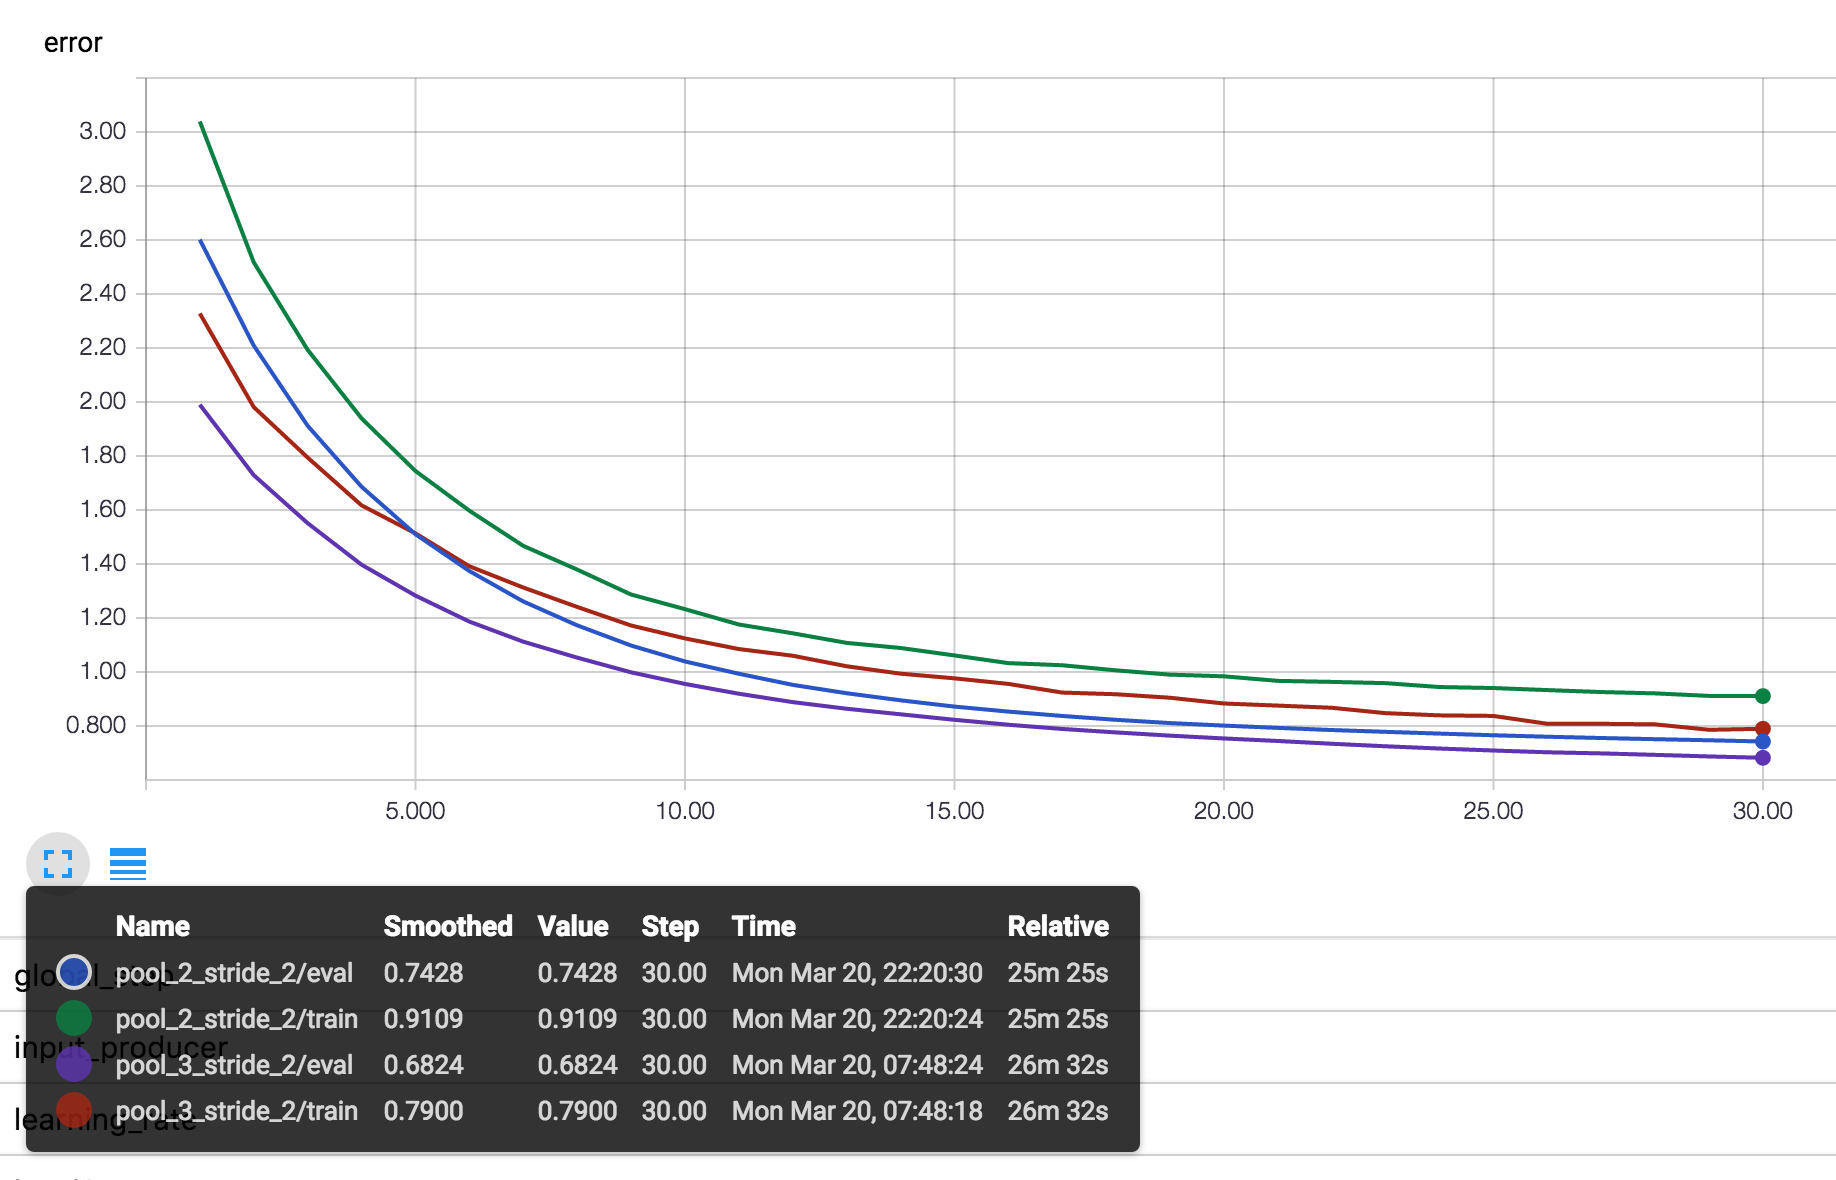
\includegraphics[width=1.0\linewidth]{poole.png}
    \end{subfigure}
    \caption{Comparison of two standard pooling parameters 2x2 and 3x3 with stride 2.}
    \label{fig:pool}
\end{figure*}


Max pooling has been shown to be very advantageous however the standard approaches usually reduce the input size by a factor of 2 which might be too rapid. One paper\cite{frac} suggests replacing max pooling with fractional pooling that allows to decrease the input size by an non integer factor for example $\sqrt{2}$. This would allow to have essential twice as many convolutional and pooling layers each viewing the input image at a different scale. Fractional pooling was implemented using \textit{tf.nn.fractional\_ max\_ pool()} and tested with different parameters allowing for a different number of pooling layers based on how quickly they decrease the input size as shown in Table \ref{tab:convpoolpar}. And the pooling region choice was set to pseudo-random as the paper suggests for models which use data augmentation.


\begin{table}[H]
\centering
\begin{tabular}[h]{| c | c |}
\hline
Pooling parameter & Pooling layers  \\
\hline
1.4 & 6   \\
\hline
1.7 & 5  \\
\hline
2.1 & 3   \\
\hline 
2.4 & 2   \\
\hline 
\end{tabular} 
\caption{Fractional pooling parameters}
\label{tab:fracpool}
\end{table}

The fractional pooling results are displayed on Figure \ref{fig:fracpool}.

\begin{figure*}[ht!]
    \centering
    \begin{subfigure}[t]{0.475\textwidth}
        \centering
        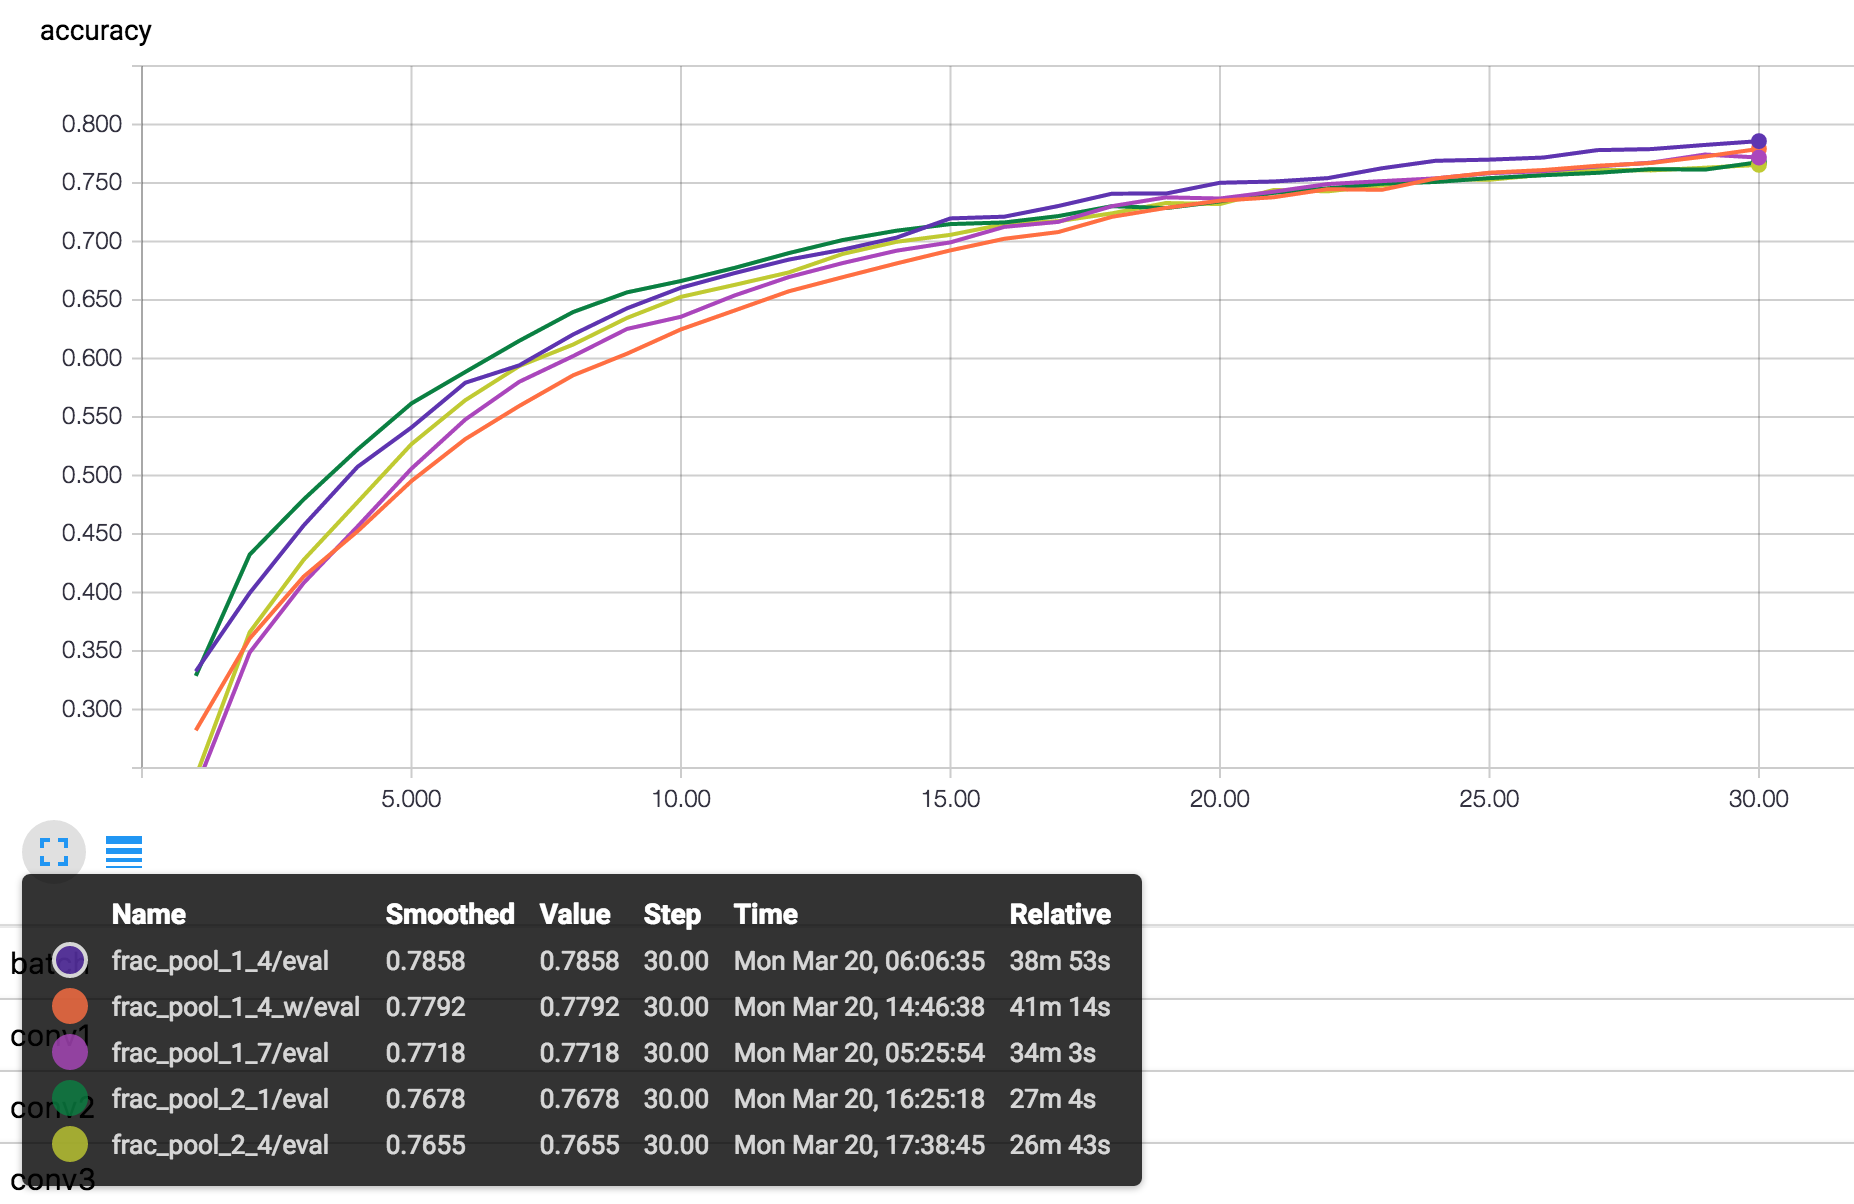
\includegraphics[width=1.0\linewidth]{fraca.png}
    \end{subfigure}%
    ~ 
    \begin{subfigure}[t]{0.475\textwidth}
        \centering
        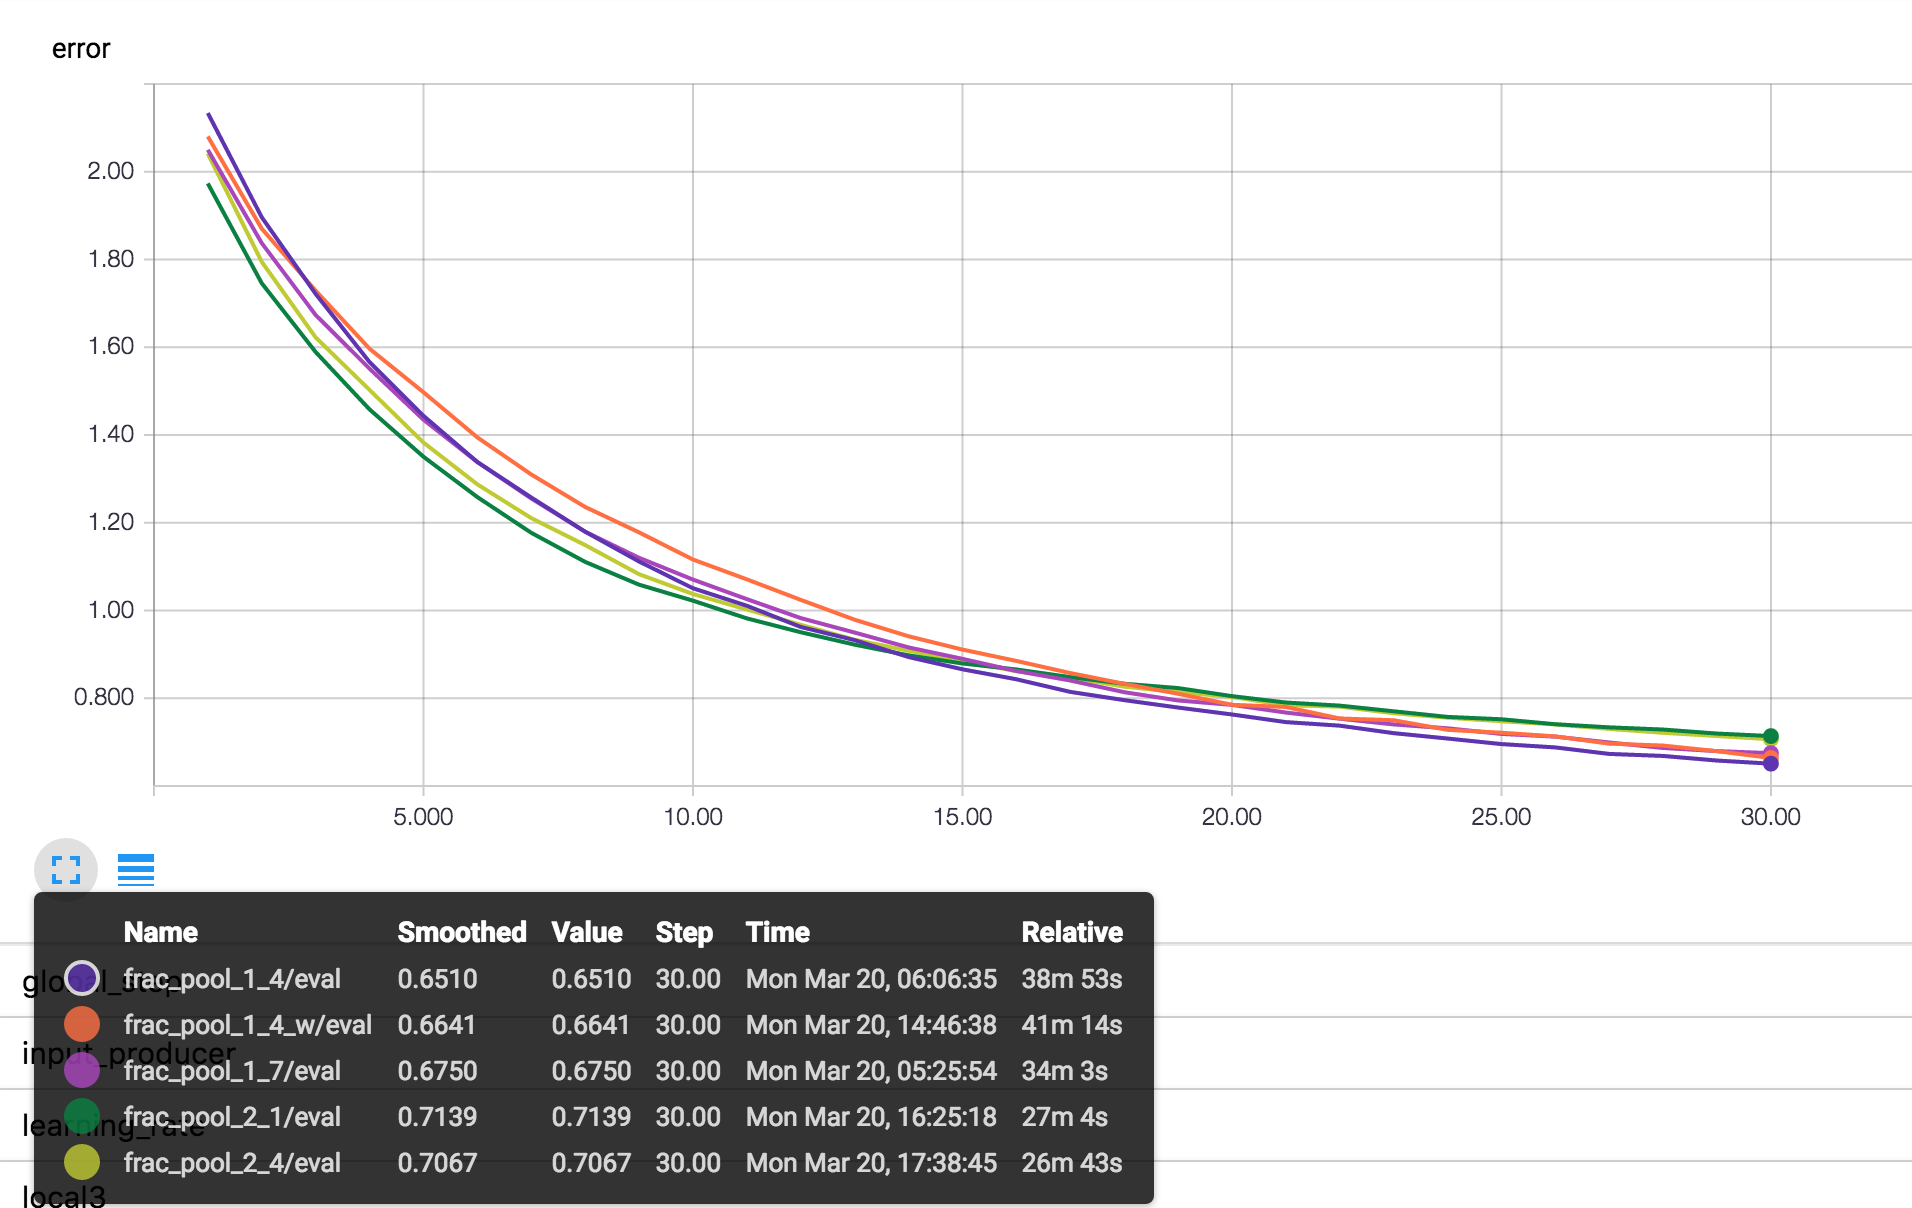
\includegraphics[width=1.0\linewidth]{frace.png}
    \end{subfigure}
    \caption{Fractional pooling performance with different parameters and number of layers. }
    \label{fig:fracpool}
\end{figure*}

\subsubsection*{The all conovolutional network}

This section is inspired by the starving for simplicity: The all convolutional network paper \cite{allconv}. The paper challenges the standard widely used pipeline of convolutional, pooling and fully connected layers. Suggesting that max pool layers can be replaced by a convolutional layer with a stride 2 to achieve the same result. An advantage is that since the input size is not being reduced (a problem fractional pooling was trying to address), allowing to build deeper networks. Implementation in tensorflow meant replacing the existing maxpool layers with conv2d layers with a stride 2. The architecture is the paper proposed All-CNN-C as described in Table \ref{tab:allcnn}. 

\begin{figure*}[ht!]
        \centering
        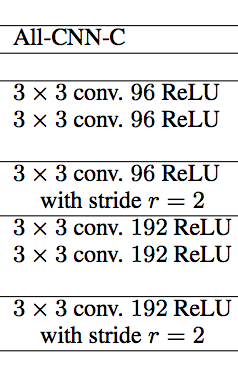
\includegraphics[width=0.17\linewidth]{allcnnc.png}
    \caption{The All-CNN-C architecture}
    \label{tab:allcnn}
\end{figure*}

The comparison of performances between our found best performing model and and the all convolutional network can be seen on Figure 

\subsection*{Discussion}

An acknowledged limitation of the experiments performed was the rather small number of 30 epoch. Due to computational and time complexity it was not perform all of these with a larger number of epochs, with the hopes that the trends would be apparent even with this smaller number.

\subsubsection*{Network architecture}

The network architecture section shows a clear motivation for using conovlutional neural networks compared to just network with fully connected layers explored in the previous assignment. Multiple iterations of convolution and pooling layers followed by fully connected layers were explored. More convolutional and pooling layers allowed the network to learn features and feature of features of the images, allowing to learn features like corners or edges. The larger number of of these convolutional layers proved to be beneficial to a cut off point when the input size became too small for convolutional filters. Increasing the number of fully connected layers following these beyond 2 did not improve the results likely due to the small input entering them. The comparison of our previously found model\cite{me} and the 3 convolution/pooling layer followed by 2 fully connected layers is shown on Figure \ref{fig:netcomp}. The advantages of conolutional networks were expected as per a large number of papers reporting positive results\cite{{inspiration}}\cite{alexnet}\cite{stan}.

\begin{figure*}[ht!]
    \centering
    \begin{subfigure}[t]{0.475\textwidth}
        \centering
        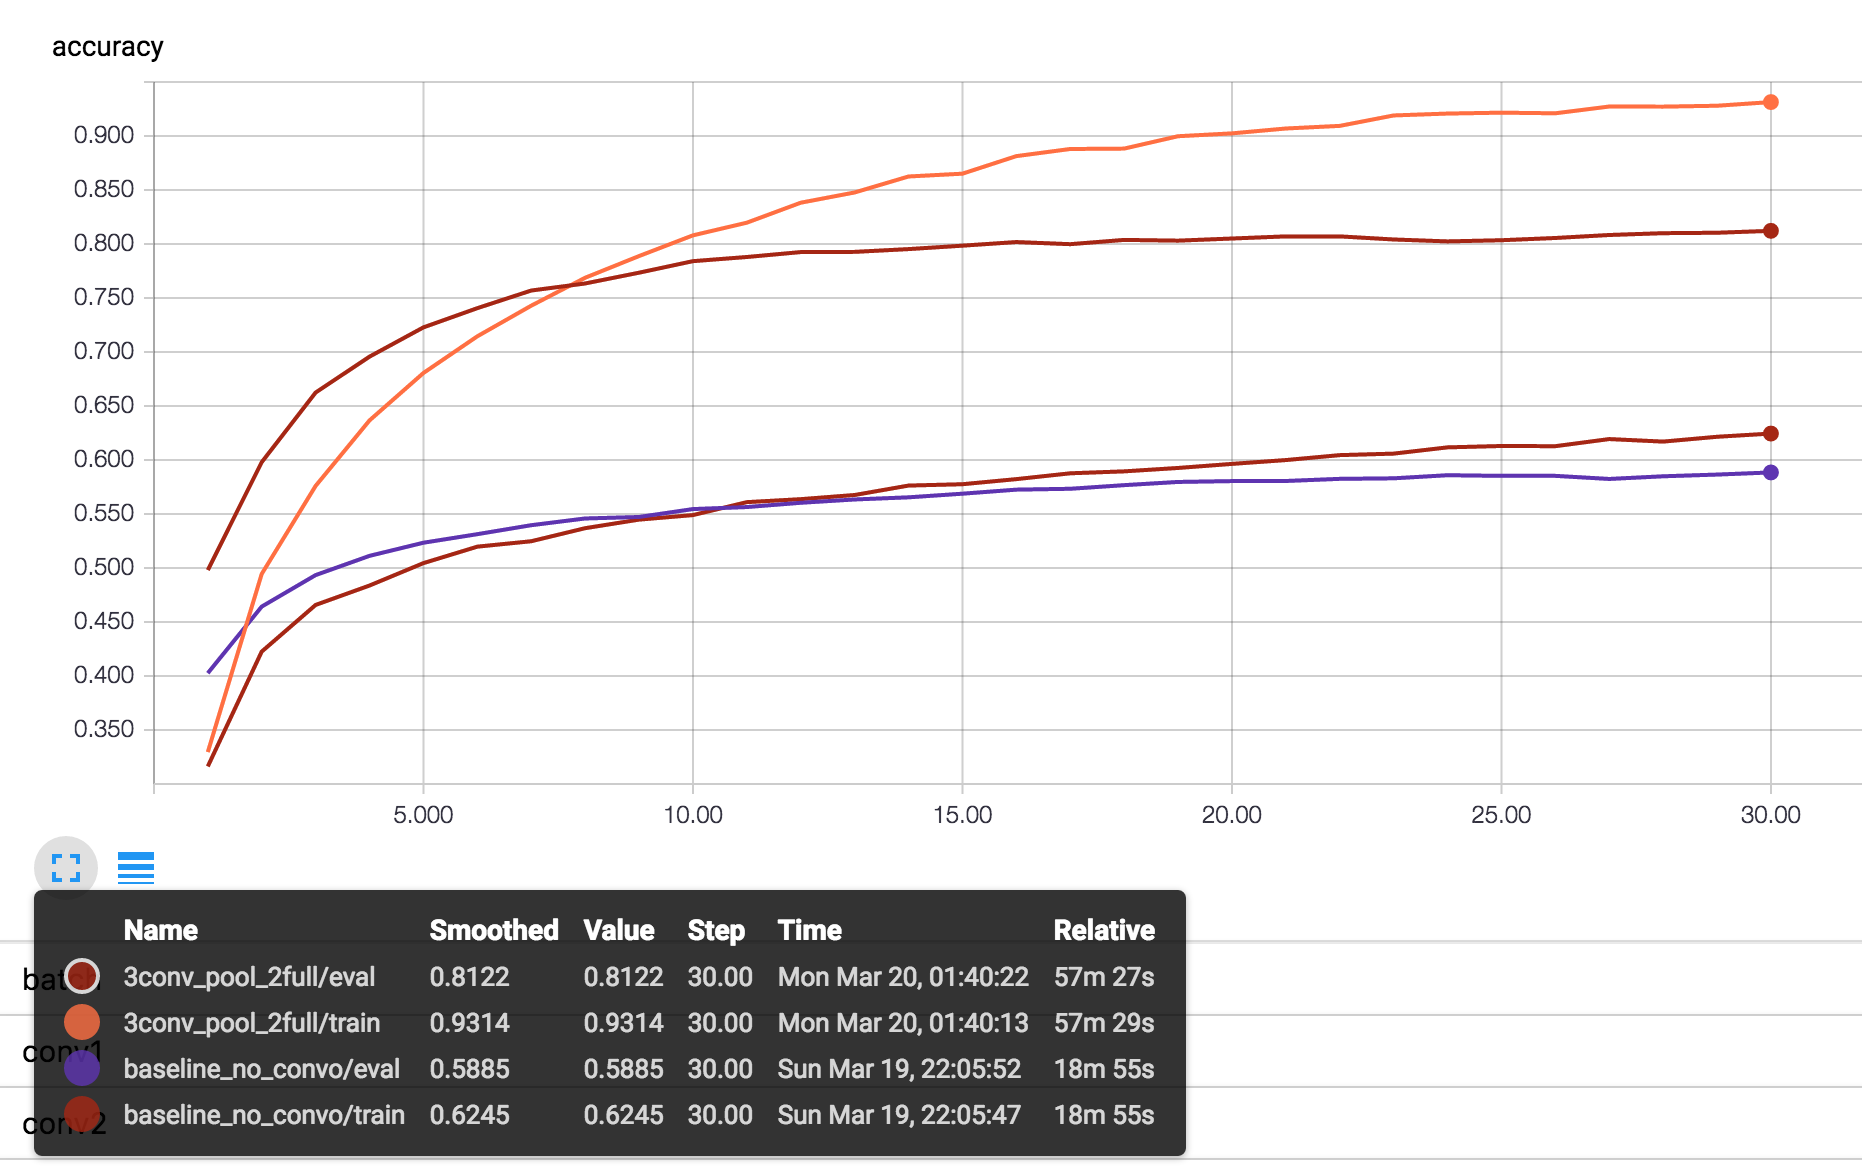
\includegraphics[width=1.0\linewidth]{netcompa.png}
    \end{subfigure}%
    ~ 
    \begin{subfigure}[t]{0.475\textwidth}
        \centering
        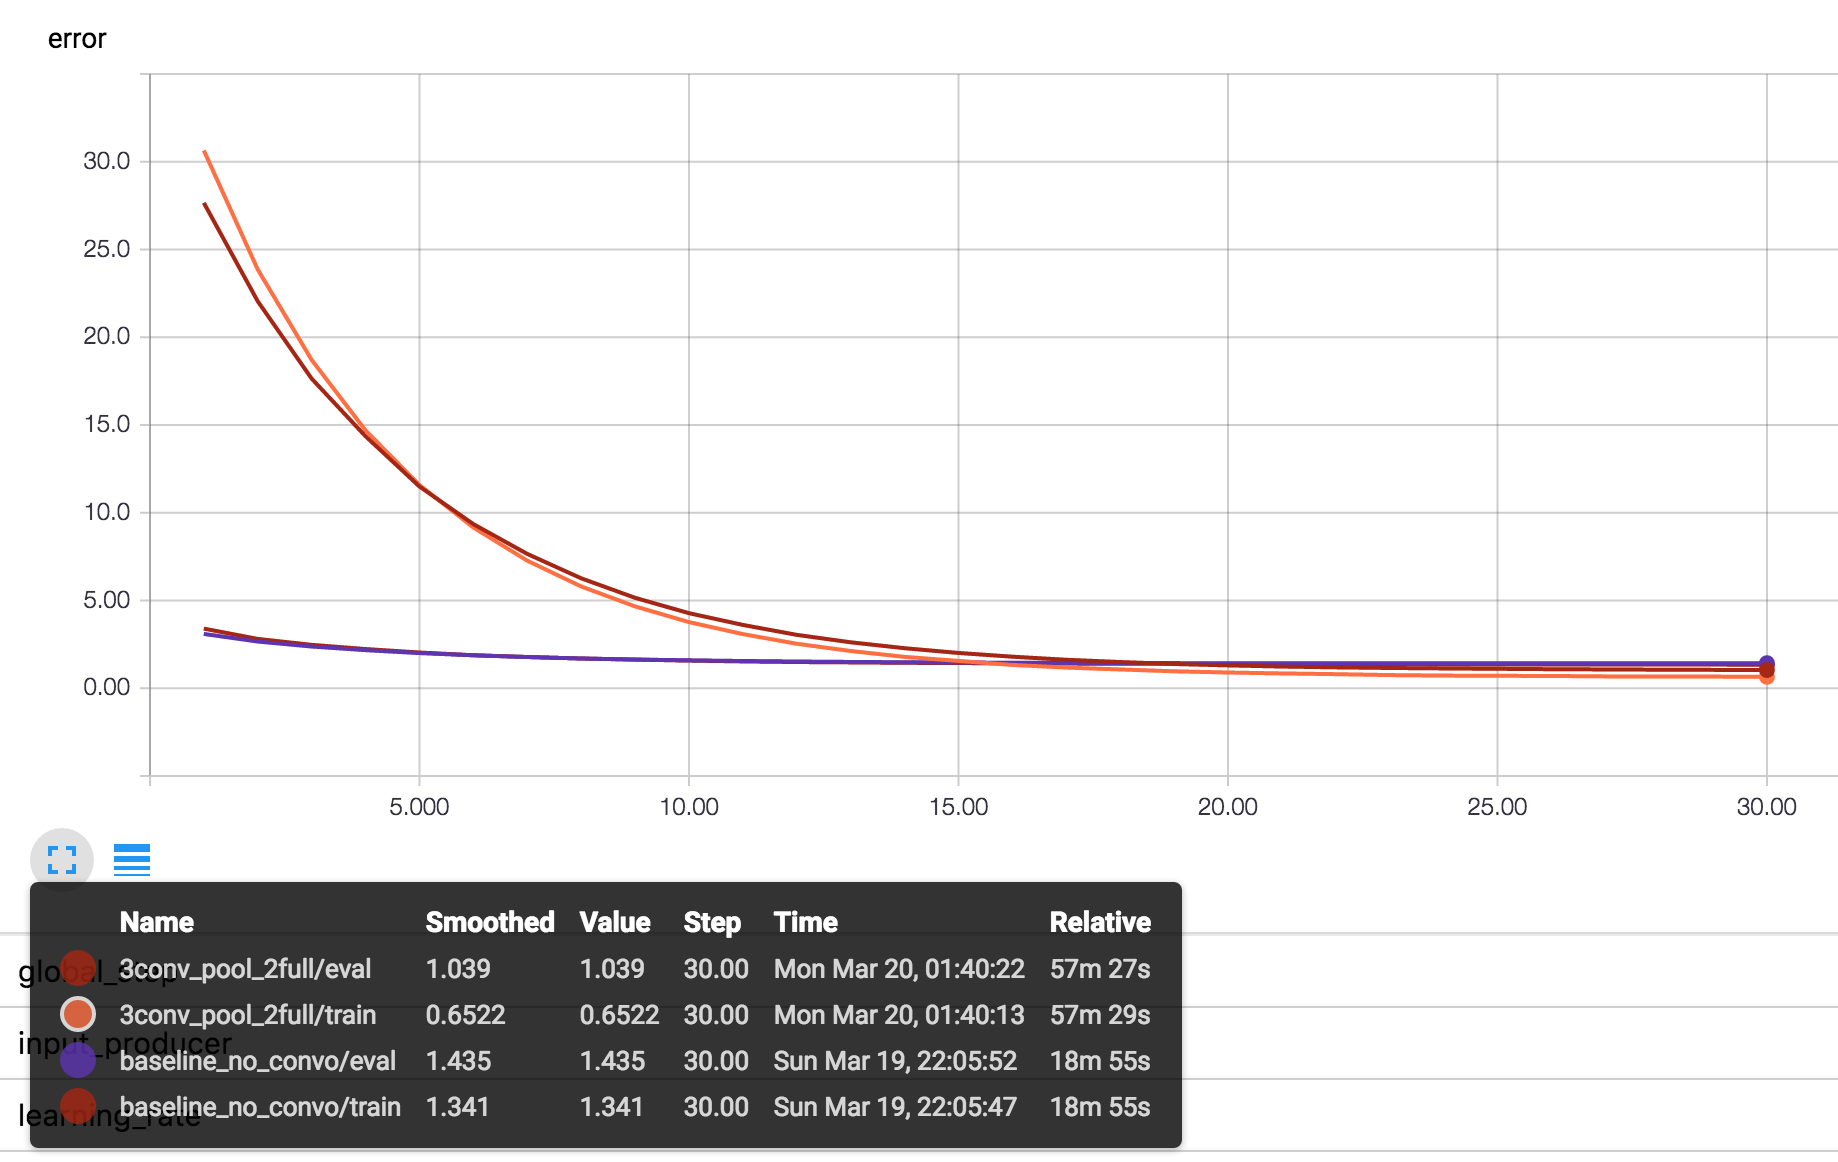
\includegraphics[width=1.0\linewidth]{netcompe.png}
    \end{subfigure}
    \caption{Comparison of baseline and conovlutional network}
    \label{fig:netcomp}
\end{figure*}

\subsubsection*{Data Augmentation}

As can be observed from Figure \ref{fig:netcomp} the conolutional model was still prone to overfitting despite the number of data augmentation methods already applied. One popular method that was not applied was random cropping used by many papers\cite{kernel}\cite{crop}. This method is able to mimic a significantly larger dataset and the results are on Figure \ref{fig:augcomp}. These show a small increase in performance over the small number of epochs but more importantly by a larger essentially larger dataset the model was no longer overfitting, which should be even more apparent with a larger number of epochs ran. The reported results confirm the initial hypothesis of this being an effective data augmentation method as was suggested by the papers.

\begin{figure*}[ht!]
    \centering
    \begin{subfigure}[t]{0.475\textwidth}
        \centering
        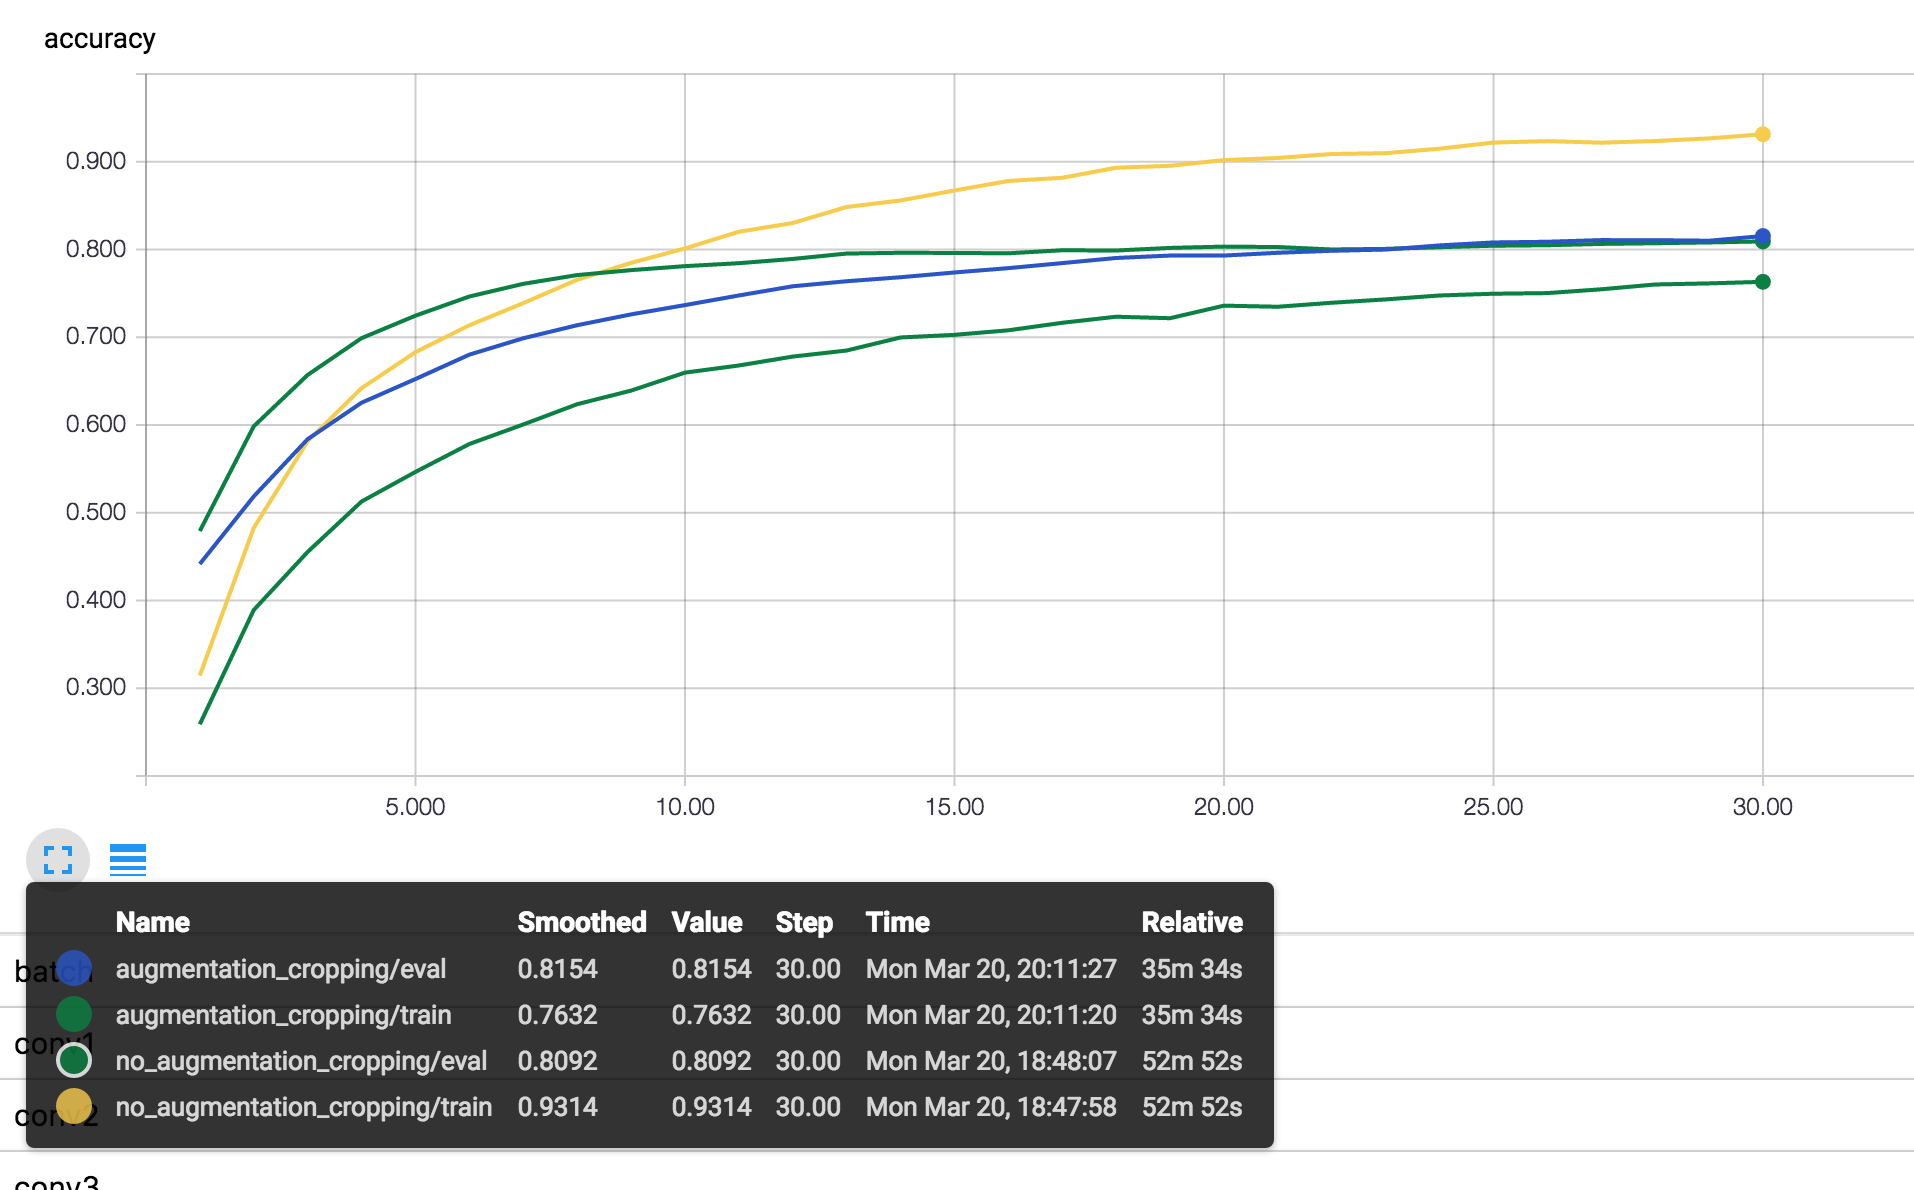
\includegraphics[width=1.0\linewidth]{disauga.png}
    \end{subfigure}%
    ~ 
    \begin{subfigure}[t]{0.475\textwidth}
        \centering
        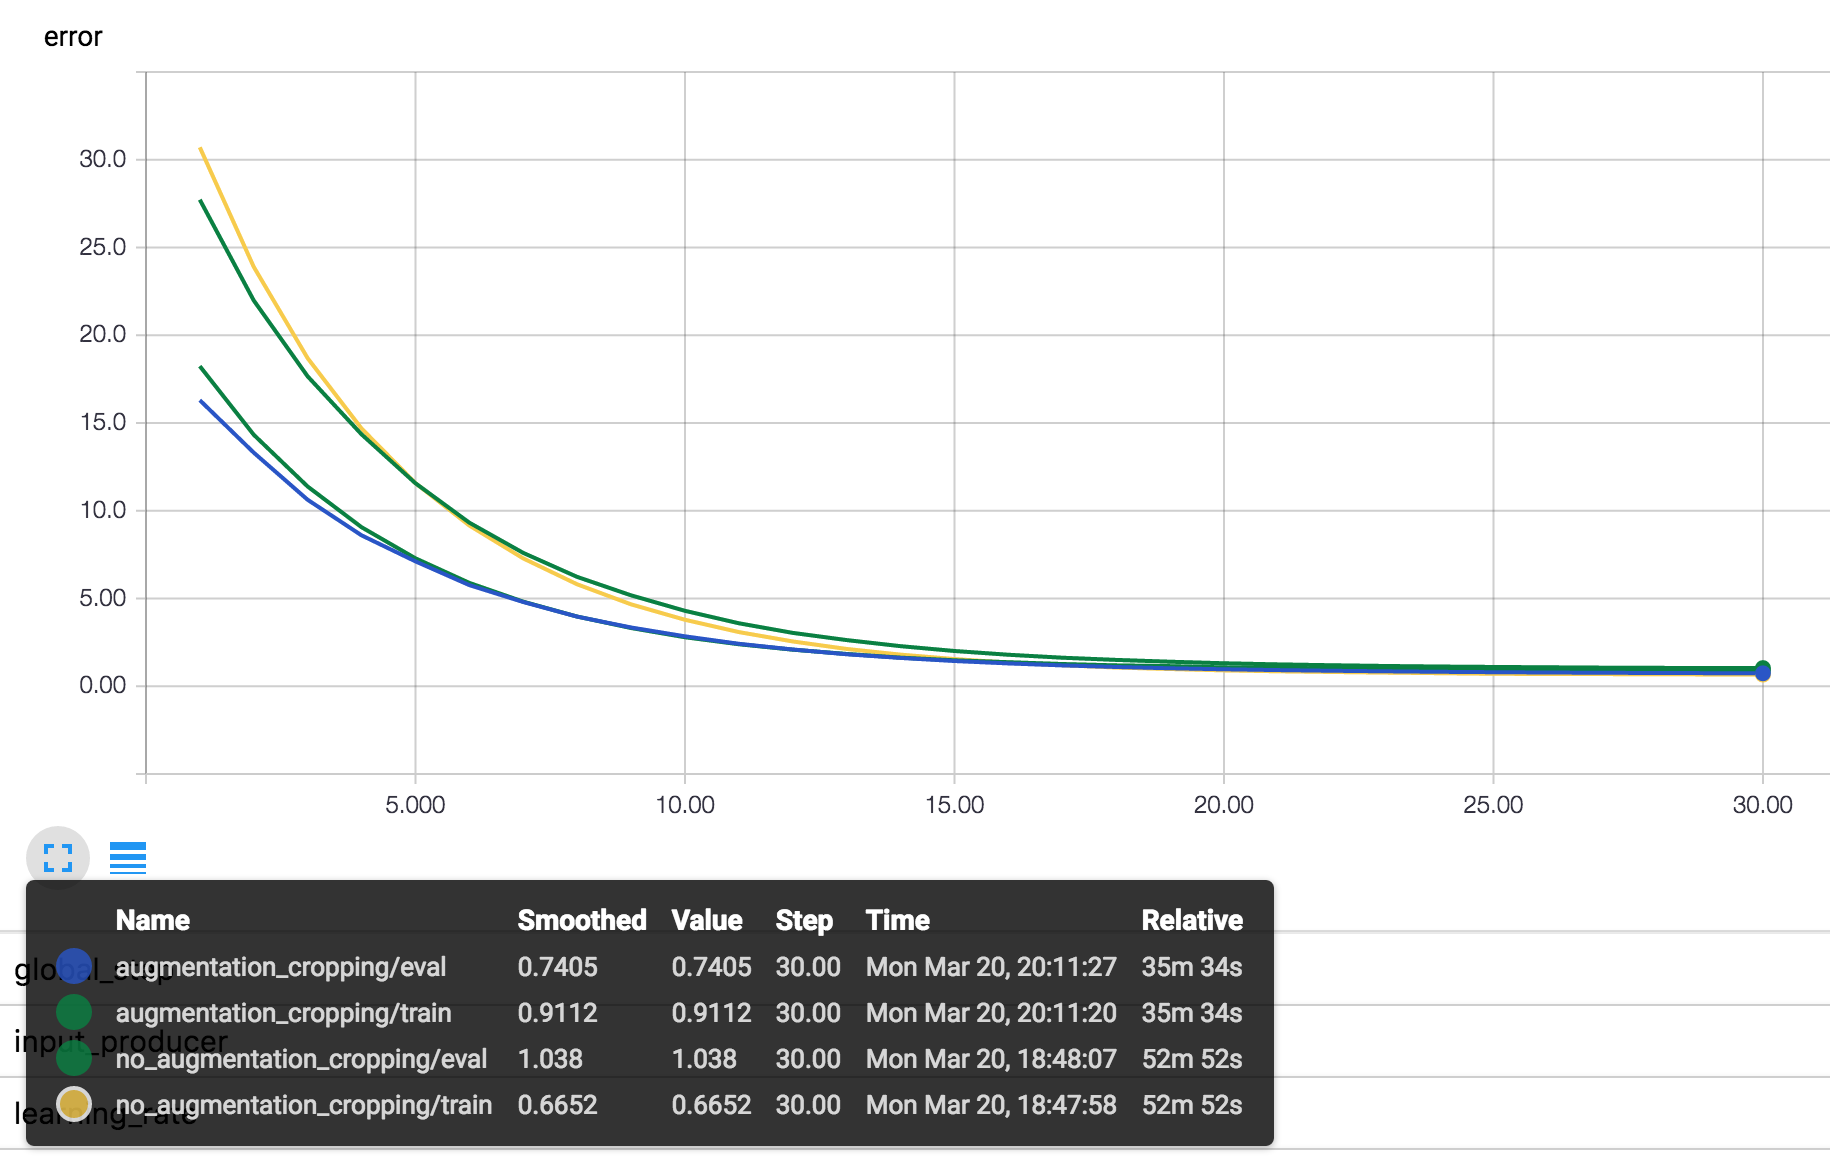
\includegraphics[width=1.0\linewidth]{disauge.png}
    \end{subfigure}
    \caption{Effects of using random cropping}
    \label{fig:augcomp}
\end{figure*}

\subsubsection*{Convolution filter size and stride length}

This section aimed to confirm the generally accepted values\cite{kernel}\cite{inspiration}\cite{bestprac} for the filter sizes of 3x3 and 5x5. As was shown in Figure \ref{fig:filter} the results confirm this notion with respect to this dataset that these two values perform both really well, whilst increasing the filter size does not. Larger filter sizes can still be beneficial\cite{alexnet} mainly in cases with larger input sizes. Increasing stride length did not improve the results as at that point the convolutional filters starts behaving more like a polling layer. Further experiments could have explored varying filter sizes, having a larger filter size in the first layer and a small one at the last one. 

\subsubsection*{Pooling kernel size, stride length and fractional pooling}

As with the section above the aim was to first explore the two generally used values for pooling 2x2 and 3x3 with stride 1 and 2 respectively. The expected results were that the 3x3 overlapping pooling will outperform the 2x2 as mentioned in some papers\cite{inspiration}\cite{frac}. The results on Figure \ref{fig:pool} reported similar performances. The larger pooling kernel size was expected to improve generalization, however due to a limited number of epoch and effective data augmentation this might have not became apparent. 



Fractional pooling\cite{frac} was then explored which allowed to reduce the size of input by a factor smaller than 2 and hence introduce more conovlutional layers. Comparison of fractional and max pooling is shown on Figure \ref{fig:fraccomp}. The results showed almost identical results, despite the expectation of fractional pooling to perform better. This could have been caused by one of two factors : the number of epochs or the different architecture used in the paper. The number of epochs was increased to 50 to explore how the models will compare, but showed no significant differences at this number. The paper described a model with conovolutional layers ending in size 1x1 and no fully connected layers. However due to similar results fractional pooling stills appears as a viable approach and could be explored further.

\begin{figure*}[ht!]
    \centering
    \begin{subfigure}[t]{0.475\textwidth}
        \centering
        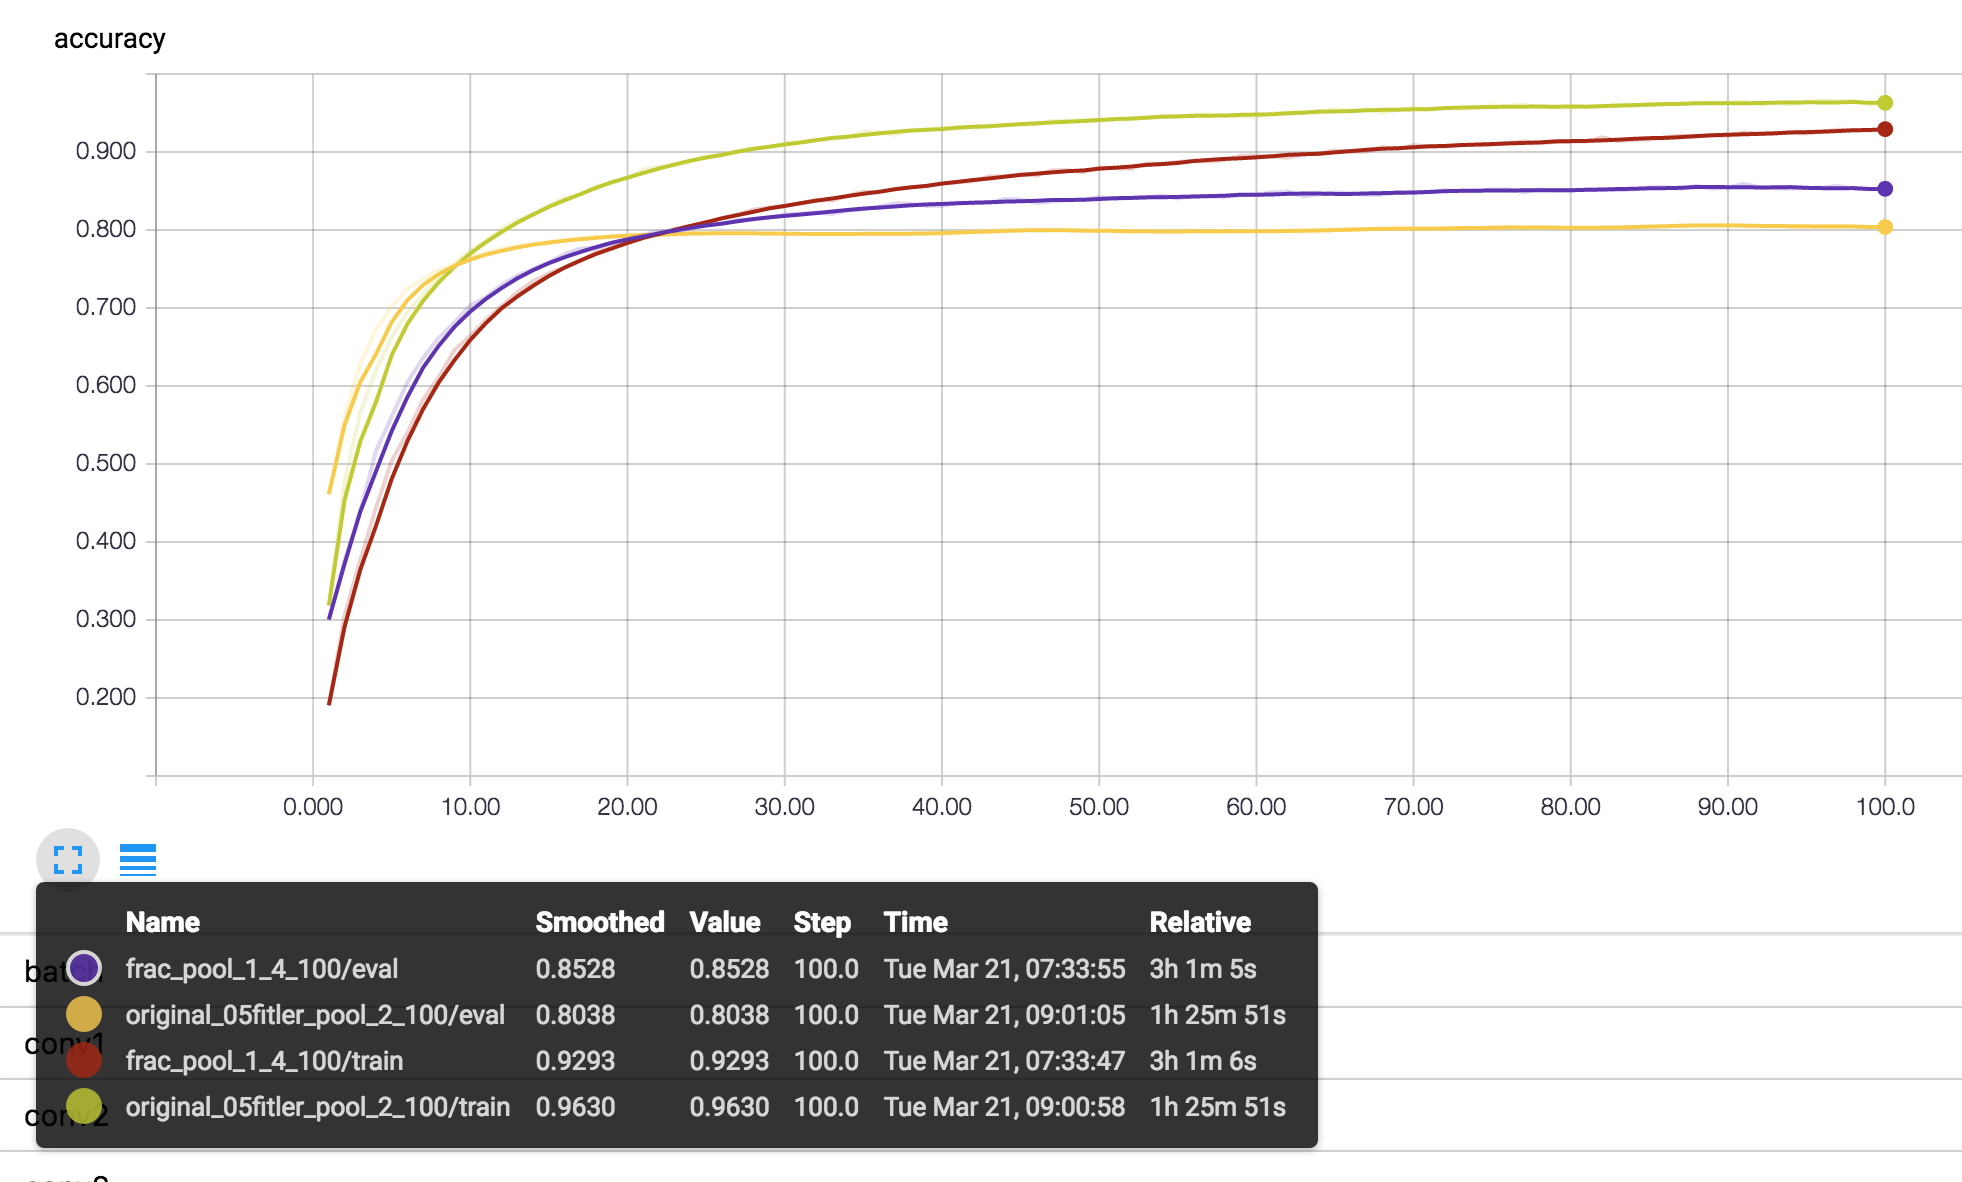
\includegraphics[width=1.0\linewidth]{disfraca.png}
    \end{subfigure}%
    ~ 
    \begin{subfigure}[t]{0.475\textwidth}
        \centering
        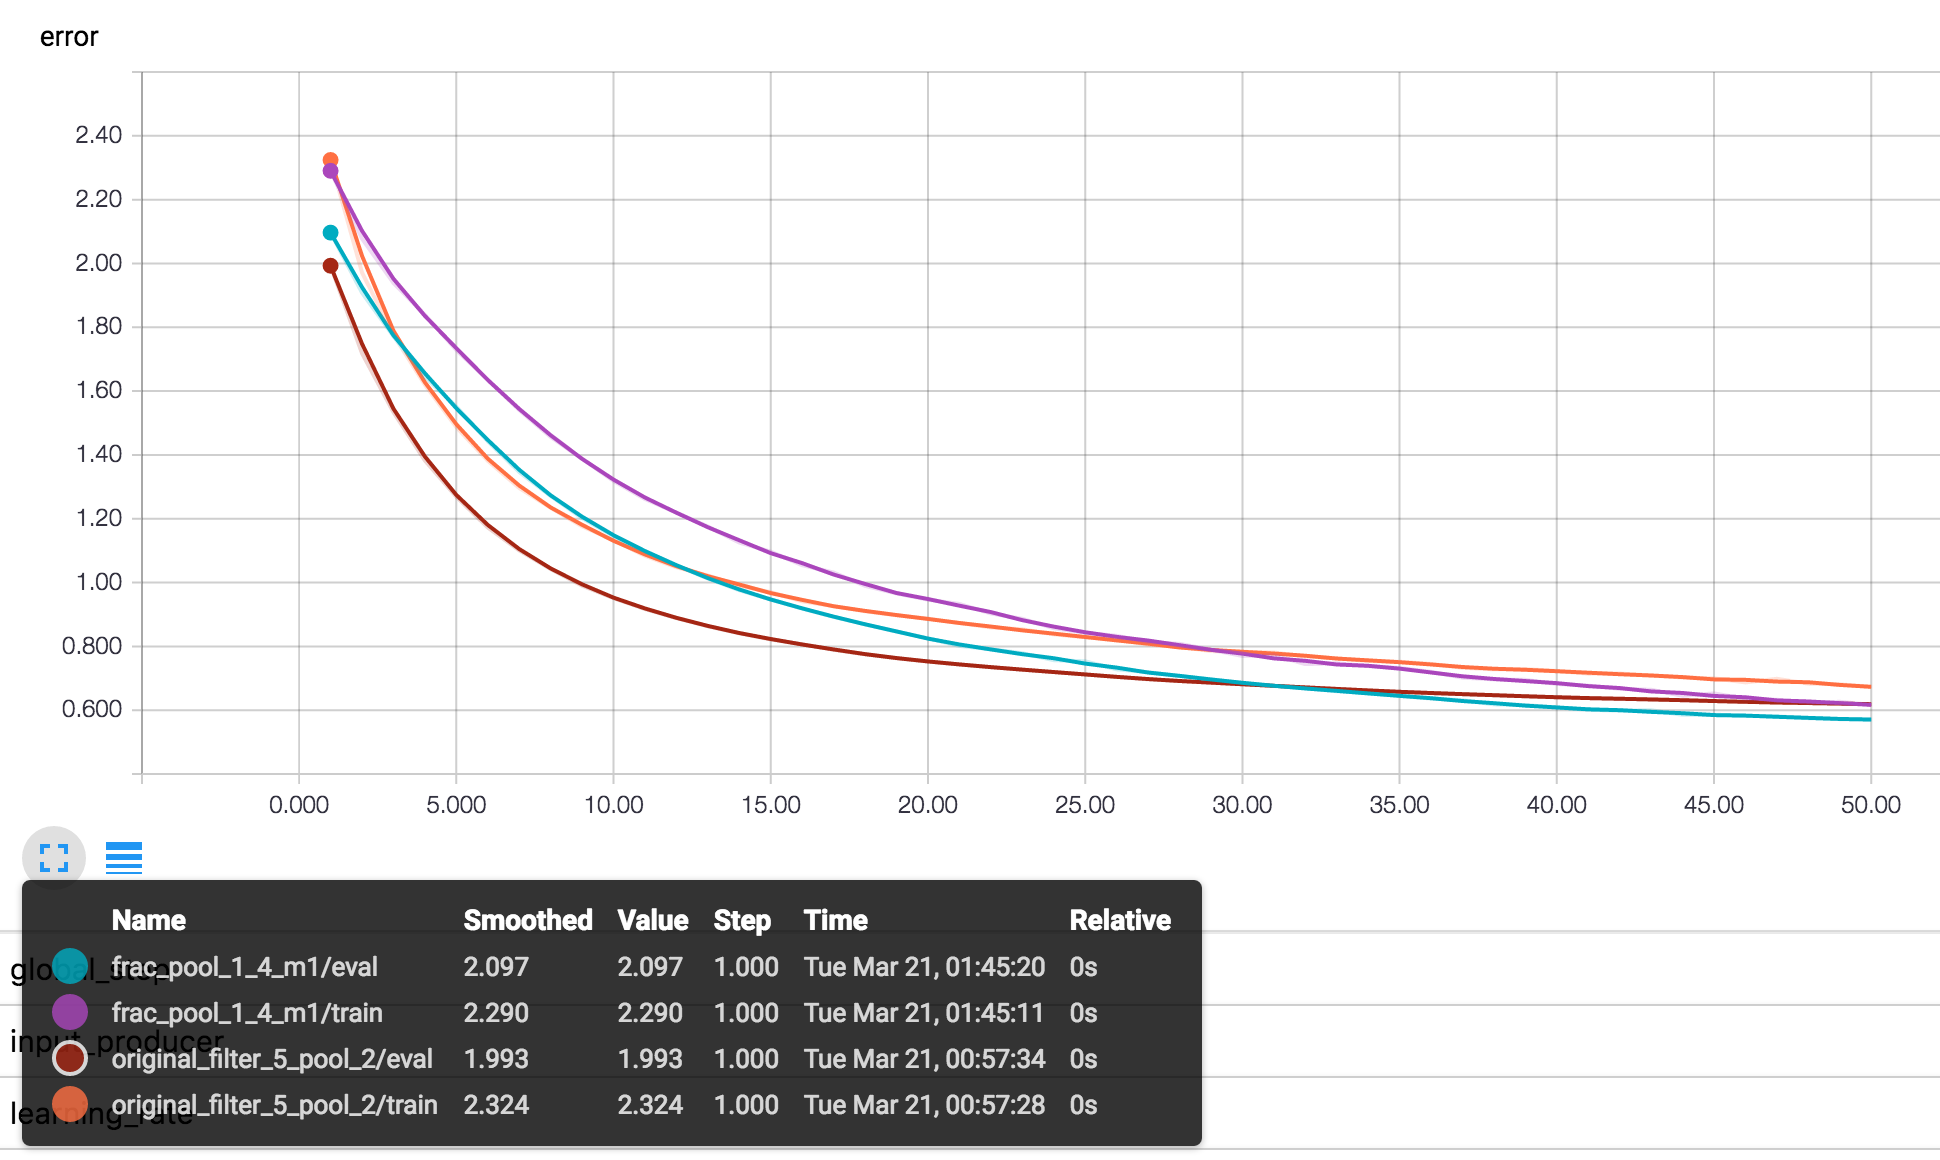
\includegraphics[width=1.0\linewidth]{disfrace.png}
    \end{subfigure}
    \caption{Comparison of fractional and max pooling.}
    \label{fig:fraccomp}
\end{figure*}

\subsection{The all conovolutional network}

The all convolutional network\cite{allconv} is an interesting approach which replaces pooling layers with conovlutional layers with stride 2. Suggesting that it might replace and simplify the standard convolutional neural network pipeline\cite{stan}. The paper reported very positive results on CIFAR and hence was explored in this setting and compared to the previously explored models. The architecture was directly adapted from the paper, but the data with augmentations is the same as with previously explored models for comparison purposes. The results confirm the paper's suggestions showing slightly improved results over our best found model so far, trained on 50 epochs for little more reliable results as shown on Figure \ref{fig:allcomp}. Further architectures in terms of number of layers, filter sizes and depths could be explored. 

\begin{figure*}[ht!]
    \centering
    \begin{subfigure}[t]{0.475\textwidth}
        \centering
        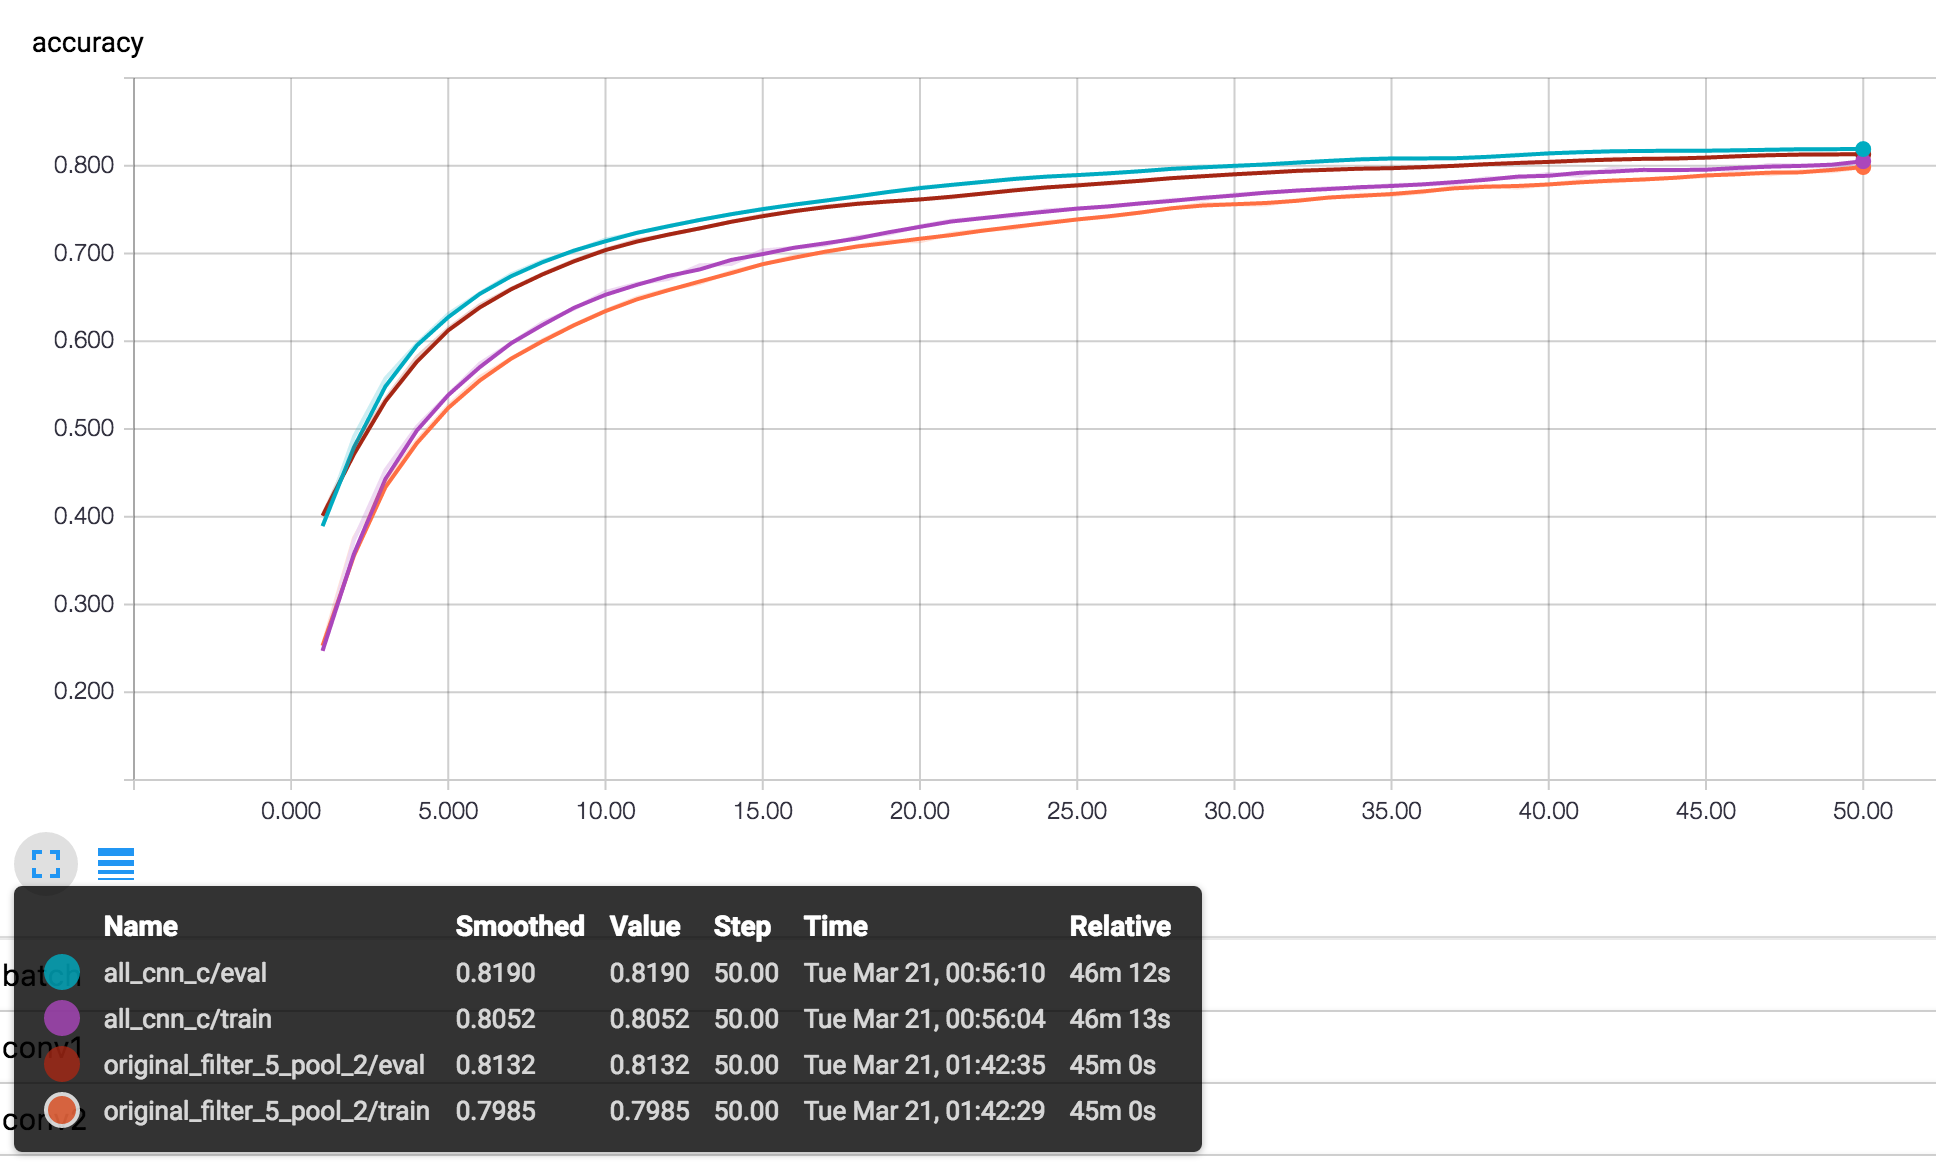
\includegraphics[width=1.0\linewidth]{disalla.png}
    \end{subfigure}%
    ~ 
    \begin{subfigure}[t]{0.475\textwidth}
        \centering
        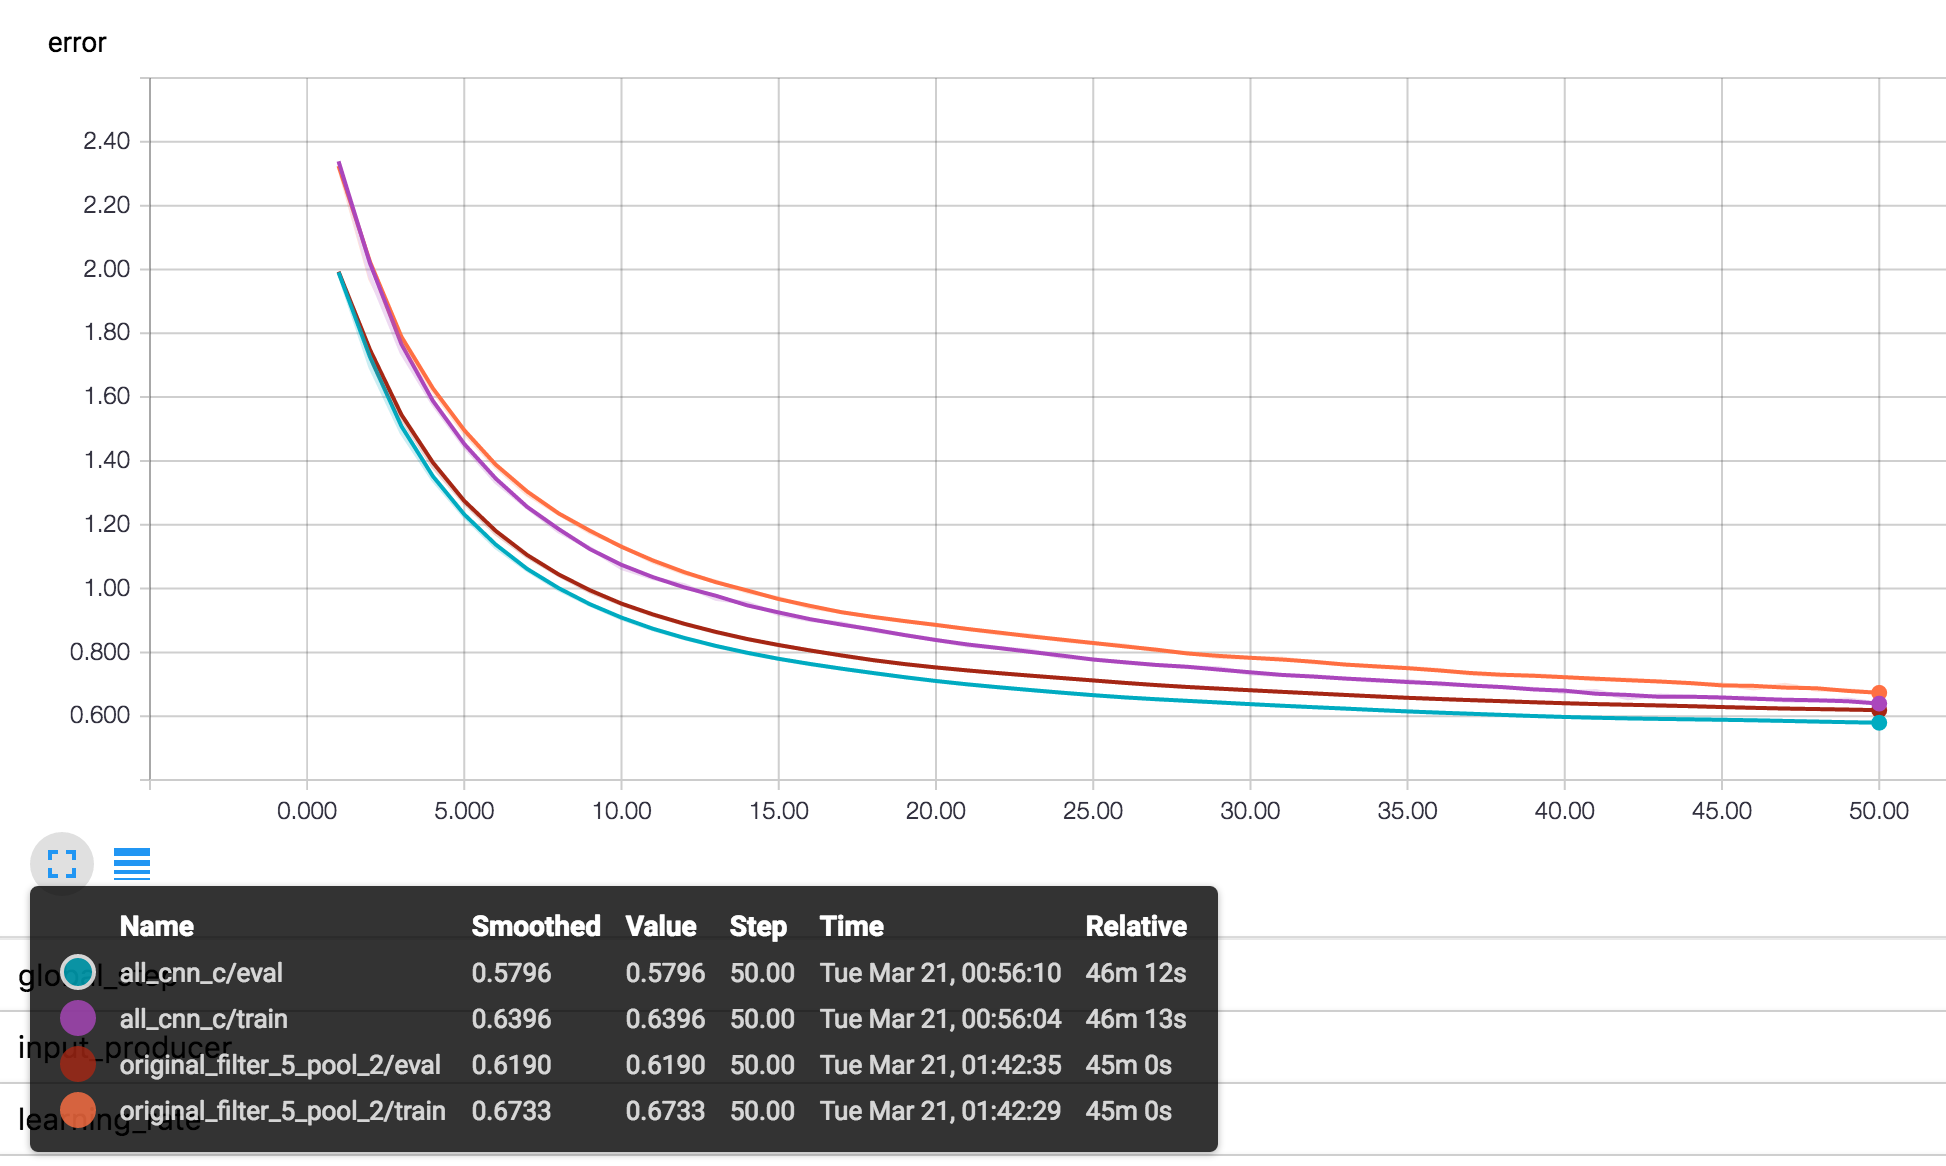
\includegraphics[width=1.0\linewidth]{disalle.png}
    \end{subfigure}
    \caption{Comparison of all convolutional network and the standard explored pipeline.}
    \label{fig:allcomp}
\end{figure*}

\subsection*{Overall}

The comparison of the three found best performing models with the baseline are shown on Figure \ref{fig:rescomp}. These models are 3(C-MP2) 2FC(200), 3(C-FP1.4)-2FC(200) and All-CNN-C. All three display similar performance on the rather small 50 number of epochs but a significant improvement over the baseline model. The best performing model was the All-CNN-C, with some potential of improvement as it has not been explored fully. 

\begin{figure*}[ht!]
    \centering
    \begin{subfigure}[t]{0.475\textwidth}
        \centering
        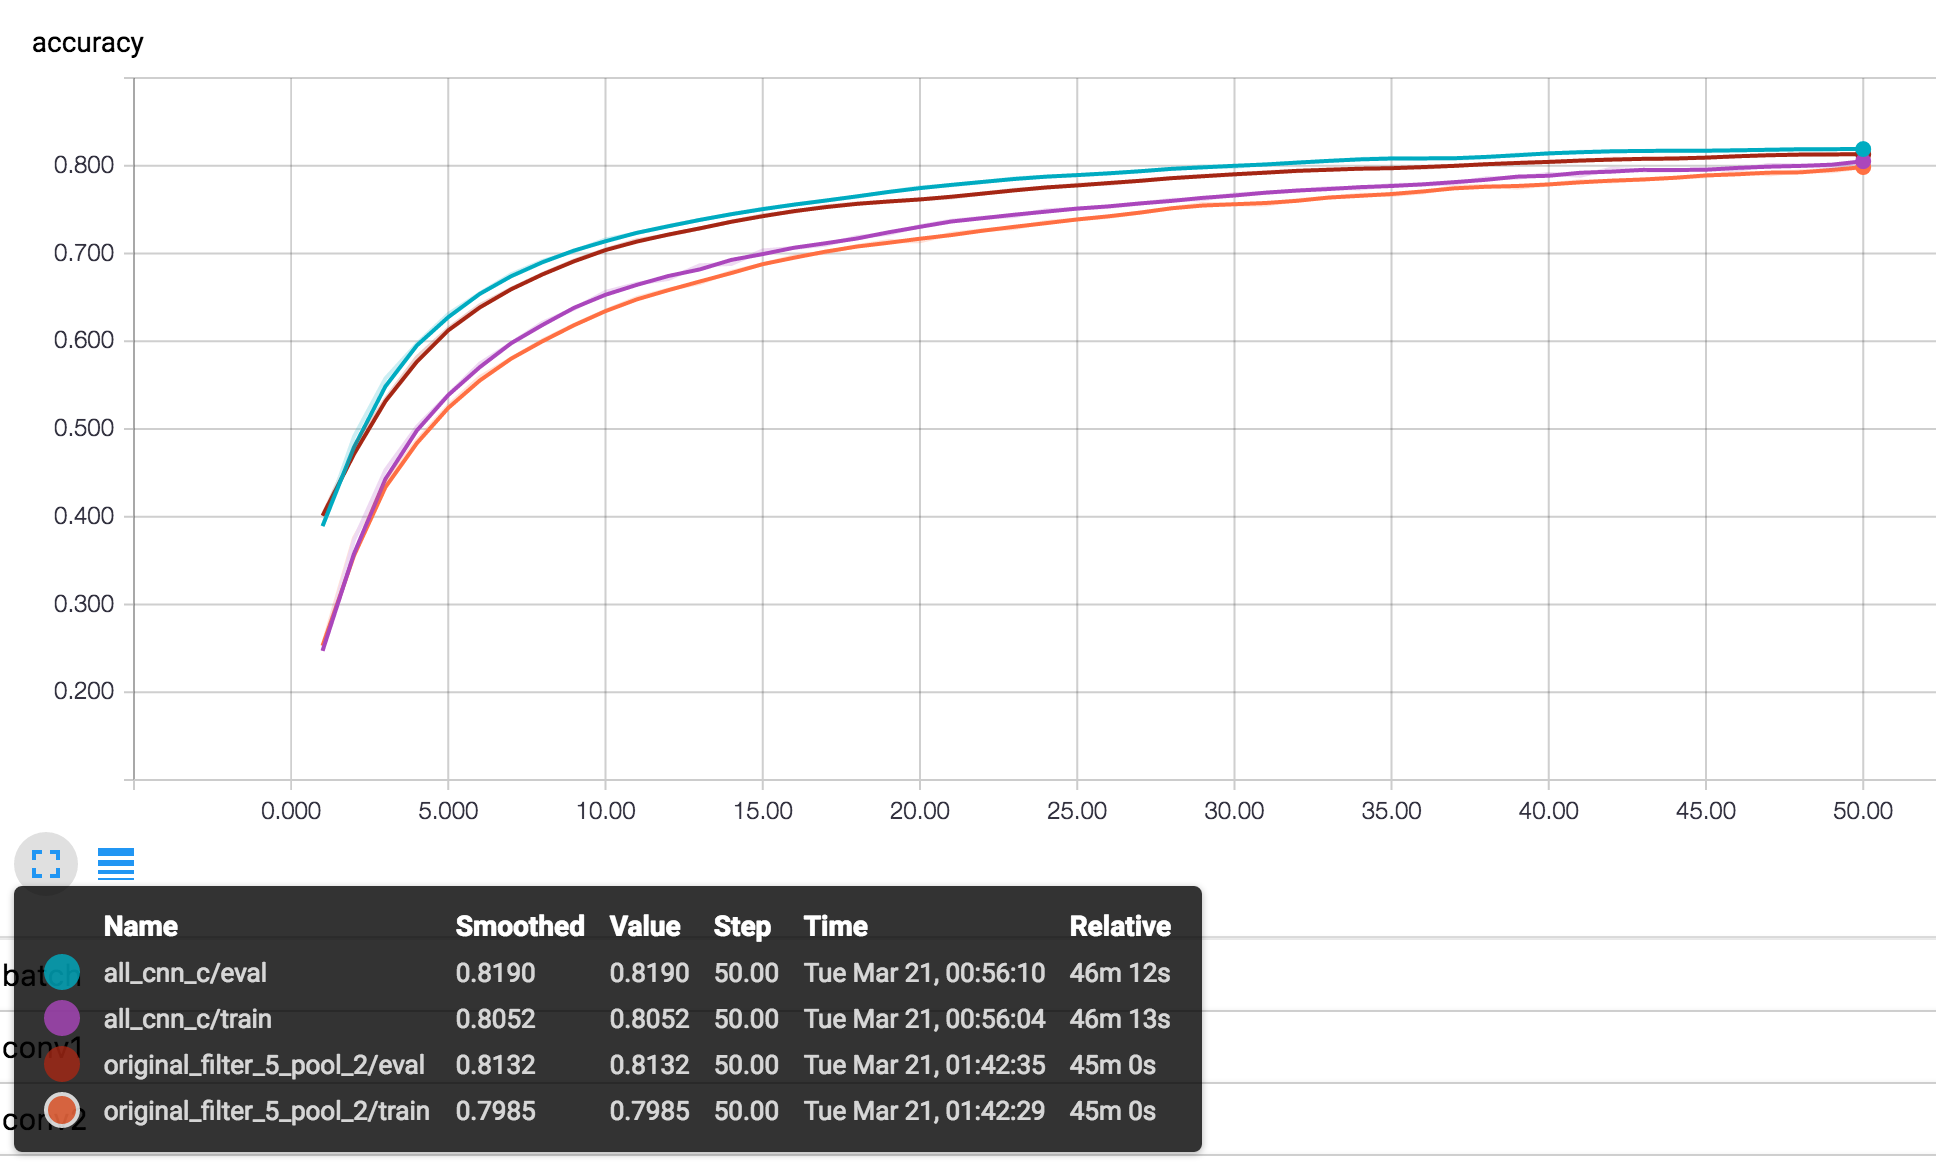
\includegraphics[width=1.0\linewidth]{disalla.png}
    \end{subfigure}%
    ~ 
    \begin{subfigure}[t]{0.475\textwidth}
        \centering
        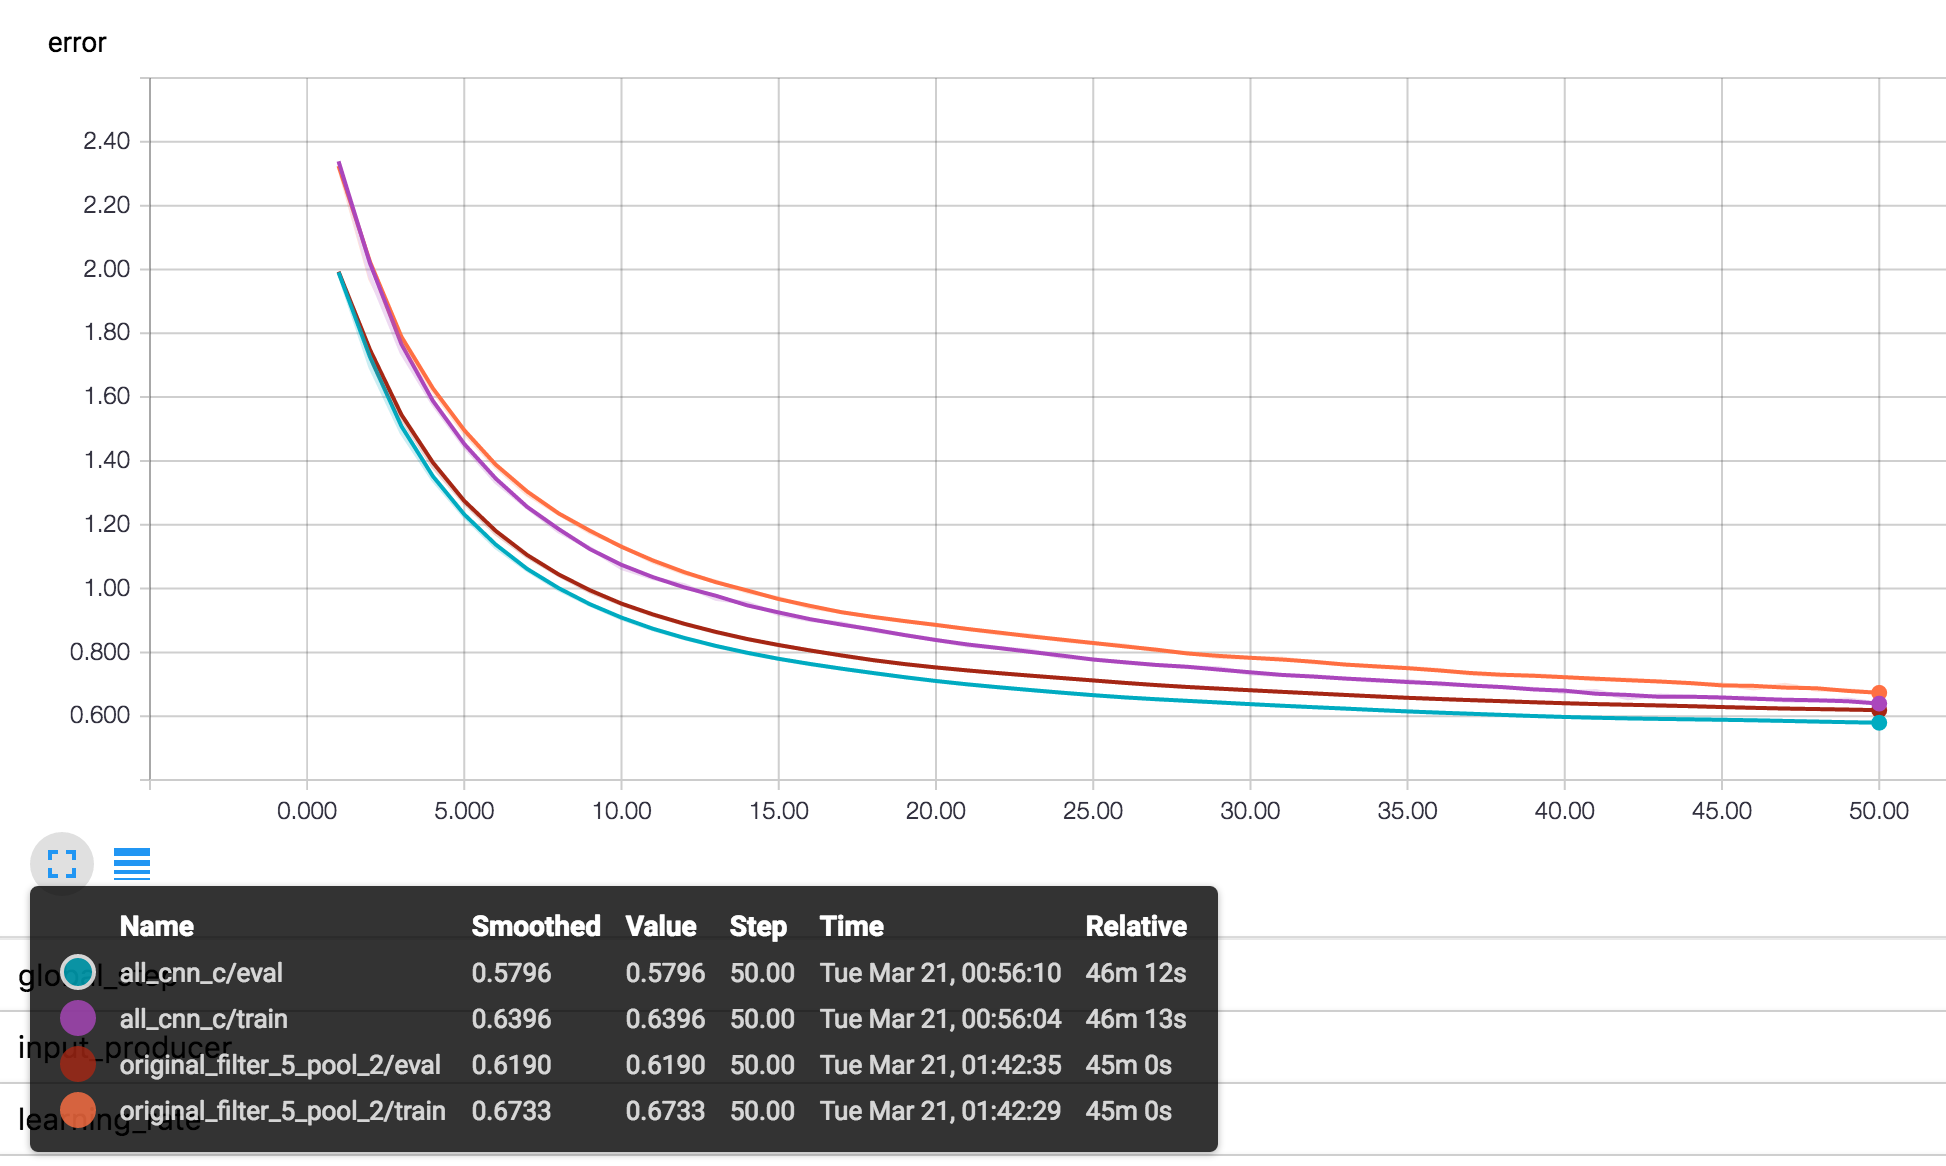
\includegraphics[width=1.0\linewidth]{disalle.png}
    \end{subfigure}
    \caption{Comparison of the best performing models explored with baseline.}
    \label{fig:rescomp}
\end{figure*}


\begin{thebibliography}{1}
\bibitem{me} s1247438 {\em Machine Learning Practical - Assignment 3}, 2017 
\bibitem{inspiration} G. E. Hinton, N. Srivastava, A. Krizhevsky, I. Sutskever and R. R. Salakhutdinov, {\em Improving neural networks by preventing co-adaptation of feature detectors}, 2012
\bibitem{kernel} Matthew D. Zeiler, Rob Fergus {\em Stochastic Pooling for Regularization of Deep Convolutional Neural Networks},2013
\bibitem{bestprac} Patrice Y. Simard, Dave Steinkraus, John C. Platt {\em Best Practices for Convolutional Neural Networks Applied to Visual Document Analysis}, 2003
\bibitem{frac} Benjamin Graham {\em Fractional Max-Pooling}, 2015
\bibitem{tf} Convolutional Neural Networks, https://www.tensorflow.org/tutorials/deepcnn
\bibitem{crop} Ken Chatfield, Karen Simonyan, Andrea Vedaldi, and Andrew Zisserman, {\em Return of the Devil in the Details: Delving Deep into Convolutional Nets}, 2014
\bibitem{stan} http://cs231n.github.io/convolutional-networks
\bibitem{alexnet} Alex Krizhevsky,Ilya Sutskever, Geoffrey E. Hinton {\em ImageNet Classification with Deep Convolutional Neural Networks}
\bibitem{allconv} Jost Tobias Springenberg, Alexey Dosovitskiy, Thomas Brox, Martin Riedmiller {\em STRIVING FOR SIMPLICITY: THE ALL CONVOLUTIONAL NET}, 2015




\end{thebibliography}

\end{document}
